% smrdoc.tex V2.10, 13 July 2012

\documentclass[times, doublespace]{smrauth}

\usepackage{moreverb}
\usepackage{multirow}
\usepackage{cite}
\usepackage{listings}
\usepackage{color}
\usepackage[linesnumbered]{algorithm2e}

\usepackage[colorlinks,bookmarksopen,bookmarksnumbered,citecolor=red,urlcolor=red]{hyperref}

\newcommand\BibTeX{{\rmfamily B\kern-.05em \textsc{i\kern-.025em b}\kern-.08em
T\kern-.1667em\lower.7ex\hbox{E}\kern-.125emX}}

\newcommand{\red}[1]{\textcolor{red}{#1}}

\def\volumeyear{2015}

\begin{document}

\runningheads{Mathieu Nayrolles {\it et al.}}{A Bug Reproduction Approach Based on Directed Model Checking and Crash Traces}

\title{A Bug Reproduction Approach Based on Directed Model Checking and Crash Traces}

\author{Mathieu Nayrolles \corrauth $^,$ \footnotemark[2] $^,$ $^1$, Abdelwahab Hamou-Lhadj$^1$, Sofi\`ene Tahar$^2$ and Alf Larsson$^3$}

\address{\begin{center}$^1$ SBA Research Lab, ECE, Concordia University, Montréal, Canada \\
$^2$ ECE Department, Concordia University, Montréal, Canada \\
$^3$ PLF System Management, Ericsson, R \& D, Stockholm, Sweden\end{center}}

\corraddr{Mathieu Nayrolles. SBA Research Lab, ECE, Concordia University. Sir George Williams Campus
1455 De Maisonneuve Blvd. W.
Montreal, Quebec, Canada
H3G 1M8}

\begin{abstract}
Reproducing a bug that caused a system to crash is an important task for uncovering the causes of the crash and providing appropriate fixes. In this paper, we propose a novel crash reproduction approach that combines directed model checking and backward slicing to identify the program statements needed to reproduce a crash. Our approach, named JCHARMING (Java CrasH
Automatic Reproduction by directed Model checkING), uses information found in crash traces combined with static program slices to guide a model checking engine in an optimal way. We show that JCHARMING is efficient in reproducing  bugs from ten different
open source systems. Overall, JCHARMING is able to reproduce 80\% of the bugs used in this study in an average time of 19 minutes.

\end{abstract}

\keywords{Automatic Bug Reproduction, Dynamic Analysis,
Model Checking, Software Maintenance.}

\maketitle

\footnotetext[2]{Email: m\_nayrol@encs.concordia.ca}

\section{Introduction}

The first (and perhaps main) step in understanding the cause of a field crash is to reproduce the bug that caused the system to fail. A survey conducted with developers of major open source software systems such as Apache, Mozilla and Eclipse revealed that
one of the most valuable piece of information that can help
locate and fix the cause of a crash is the one that can help
reproduce it \cite{Bettenburg2008}.

\red{Bug reproduction is, however, a challenging task because of the limited amount of information  provided by the end users.} There exist several bug reproduction techniques. They can be grouped into two categories: (a)
On-field record and in-house replay \cite{Narayanasamy2005,Artzi2008,Jaygarl}, and (b) In-house crash explanation \cite{Manevich2004,chandra2009snugglebug}. The first category relies on
instrumenting the system in order to capture objects and other
system components at run-time. When a faulty behavior
occurs in the field, the stored objects, as well as the entire heap,
are sent to the developers along with the faulty methods to
reproduce the crash. These techniques tend to be simple to
implement and yield good results, but they suffer from two
main limitations. First, code instrumentation comes with a
non-negligible overhead on the system. The second limitation
is that the collected objects may contain sensitive information
causing customer privacy issues. The second category is
composed of tools leveraging proprietary data in order to
provide hints on potential causes. While these techniques are
efficient in improving our comprehension of the bugs, they are
not designed with the purpose of reproducing them.

\red{In previous work, we proposed a hybrid approach called JCHARMING
(Java CrasH Automatic Reproduction by directed Model
checkING) \cite{Nayrolles2015} that uses a combination of crash traces and model
checking to automatically reproduce bugs that caused field
failures.} Unlike existing techniques, JCHARMING does not
require instrumentation of the code. It does not need access to
the content of the heap either. \red{Instead, JCHARMING uses the list of functions that are output when an uncaught exception in Java
occurs (i.e., the crash trace) to guide a model checking engine
to uncover the statements that caused the crash.}

Model checking (also known as property checking) is a formal
technique for automatically verifying a set of properties of
finite-state systems \cite{Baier2008}. More specifically, this technique
builds a graph where each node represents one
state of the program and the set of properties that needs to be
verified in each state. For real-world programs, model
checking is often computationally impracticable because of
the state explosion problem \cite{Baier2008}. To address this challenge and
apply model checking on large programs, we direct the model
checking engine towards the crash using program slicing and
the content of the crash trace, and hence, reduce the search
space. When applied to reproducing bugs of seven open source  systems, JCHARMING achieved
 85\% accuracy.

This paper extends our previous work \cite{Nayrolles2015} with the following main contributions:
An extensive validation of JCHARMING by conducting experiments with three
additional systems: Mahout, Hadoop, and ActiveMQ,
bringing the total number of subject systems used to
validate our approach to 10 and the number of bugs to 30.
It should be noted that the new systems are larger compared to
Those used in \cite{Nayrolles2015}.
The accuracy of JCHARMING when applied to the 30 bugs is 80\%,
which is a slight decrease compared to the previous study.
This is explained by the fact that the new systems used in
this study are relatively larger compared to those in \cite{Nayrolles2015}.
Another important contribution of this paper is a completely redesigned
JUnit test case generation process.
This extended version of the paper also includes a detailed
analysis of additional bugs, an elaborate discussion of the
results, and an updated related work section.

The remainder of this paper is organized as follows: In Section
\ref{sec:rel-work}, we present related work on crash reproduction. In Section \ref{sec:prelimenaries}, we provide some background information on model
checking. JCHARMING is the topic of Section \ref{fig:jcarming-approach}. Section \ref{sec:cases}
is dedicated to the case study, followed by threats to validity.
We conclude the paper and sketch future directions in Section
\ref{sec:conclusion}.


\section{Related Works\label{sec:rel-work}}

In this section, we put the emphasis on how crash traces are used in crash reproduction tasks.
Existing studies can be divided into two distinct categories: (A) on-field record and in-house replay techniques \cite{Steven2000,Narayanasamy2005,Artzi2008,Roehm2015}, and (B) on-house crash understanding \cite{Jin2012,Jin2013,Zuddas2014,Chen2013a,Nayrolles2015}.

These two categories yield varying results depending on the selected approach and are mainly differentiated by the need for instrumentation.
The first category of techniques oversees -- by means of instrumentation -- the execution of the target system on the field in order to reproduce the crashes in-house, whereas tools and approaches belonging to the second category only use data produced by the crash such as the crash stack or the core dump at crash time. In the first category, tools record different types of data such as the invoked methods \cite{Narayanasamy2005}, try-catch exceptions \cite{Rossler2013}, or objects \cite{Jaygarl}. In the second category, existing tools and approaches are aimed towards understanding the causes of a crash, using data produced by the crash itself, such as a crash stack \cite{Chen2013a}, previous -- and controlled -- execution \cite{Zuddas2014}, etc.

\red{Tools and approaches that rely on instrumentation face common limitations such as the need to instrument the source code in order to introduce logging mechanisms\cite{Narayanasamy2005,Jaygarl,Artzi2008}, which is known to slow down the subject system.
In addition,  recording system behavior by means of instrumentation may yield privacy concerns.
Tools and approaches that only use data about a crash -- such as core dump or exception stack crashes -- face a different set of limitations. They have to reconstruct the timeline of events that have led to the crash \cite{Chen2013a,Nayrolles2015}. Computing all the paths from the initial state of the software to the crash point is a NP-complete problem, and may cause state space explosion \cite{Chen2013a,Clause2007}.}

In order to overcome these limitations, some researchers have proposed to
use various SMT (satisfiability modulo theories) solvers \cite{Dutertre2006}
and model checking techniques \cite{Visser2003}.
However, these techniques require knowledge that goes beyond traditional
software engineering, which hinders their adoption  \cite{Visser2004}.

It is worth mentioning that both categories share a common limitation.
It is possible for the required condition to reproduce a crash to be purely
external, i.e., the reading of a file that is only present on the hard
drive of the customer or the reception of a faulty network packet
\cite{Chen2013a, Nayrolles2015}.
Without this input, it may be challenging to reproduce the bug.



\subsection{On-field Record and In-house Replay}

Jaygarl {\it et al.} created OCAT (Object Capture based Automated Testing)
\cite{Jaygarl}.
The authors' approach starts by capturing objects created by the program when
it runs on-field in order to provide them to an automated test process.
The coverage of automated tests is often low due to lack of correctly
constructed objects. Also, the objects can be mutated by means of
evolutionary algorithms.
These mutations target primitive fields in order to create even more objects
and, therefore, improve the code coverage.
While not directly targeting the reproduction of a bug,
OCAT is an approach that was used as the main mechanism
for bug reproduction systems.

Narayanasamy {\it et al.} \cite{Narayanasamy2005} proposed BugNet, a tool that continuously records program execution for deterministic replay debugging. According to the authors, the size of the recorded data needed to reproduce a bug with high accuracy is around 10MB. This recording is then sent to the developers and allows the deterministic replay of a bug. The authors argued that with nowadays Internet bandwidth the size of the recording is not an issue during the transmission of the recorded data.

Another approach in this category was  proposed by Clause {\it et al.} \cite{Clause2007}. The approach records the execution of the program on the client side and compresses the generated data. Moreover, the approach keeps traces of all accessed documents in the operating system and also compresses.
Overall, the approach is able to reproduce on-field bugs using a file that are 70kb in average.
The minimal execution paths triggering the failure are then sent to the developer who can replay the execution on a sandbox simulating the client's environment.
This special feature of the approach proposed by Clause {\it et al.} addresses the limitation where crashes are caused by external causes. While the authors broaden the scope of reproducible bugs, their approach records a lot of data that may be deemed private such as files used for the proper operation of the operating system.

Timelapse \cite{Burg2013} also addresses the problem of reproducing bugs using external data. The tool focuses on web applications and allows developers to browse and visualize the execution traces recorded by Dolos. Dolos captures and reuses user inputs and network responses to deterministically replay a field crash. Also, both Timelapse and Dolos allow developers to use conventional tools such as breakpoints and classical debuggers. Similarly, private data are recorded without obfuscation of any sort.

Another approach was proposed by Artzi {\it et al.} and named ReCrash. ReCrash records the object states of the targeted programs \cite{Artzi2008}. The authors use an in-memory stack, which contains every argument and object clone of the real execution in order to reproduce a crash via the automatic generation of unit test cases.
Unit test cases are used to provide hints to the developers about the buggy code.
This approach particularly suffers from the limitation related to slowing down the execution.
The overhead for full monitoring is considerably high (between 13\% and 64\% in some cases).
The authors  propose an alternative solution in which they record only the methods surrounding the crash. For this to work, the crash has to occur at least once so they could use the information causing the crash to identify the methods surrounding it.

\red{Similarly to ReCrash, JRapture \cite{Steven2000} is a capture/replay tool for observation-based testing. The tool captures execution of Java programs to replay it in-house. To capture the execution of a Java program, the creators of JRapture used their own version of the Java Virtual Machine (JVM) and a lightweight, transparent capture process.
Using a customized JVM allows capturing any interactions between a Java program and the system including GUI, files, and console inputs.
These interactions can be replayed later  with exactly the same input sequence as saw during the capture phase.
However, using a custom JVM is not a practical solution. This is because, the authors' approach requires from users to install a JVM that might have some discrepancies with the original one and yield bugs if used with other software applications.
In our view,  JRapture fails at addressing the limitations caused
by instrumentation because it imposes the installation of another
JVM that can also monitor other software systems than the intended ones.
RECORE (REconstructing CORE dumps) is a tool proposed by Robler {\it et al.}.} The tool instruments Java byte code to wrap every method in a try-catch block while keeping a quasi-null overhead \cite{Rossler2013}. RECORE starts from the core dump and tries (with evolutionary algorithms) to reproduce the same dump by executing the subject program many times. When the generated dump matches the collected one, the approach has found the set of inputs responsible for the failure.

\red{The approaches presented at this point operate at code level.
There exist also techniques that focus on recording user-GUI interactions \cite{Herbold2011,Roehm2015}.}
Roehm {\it et al.} extract the recorder data using delta debugging \cite{Zeller2002}, sequential pattern mining, and their combination to reproduce between 75\% and 90\% of the submitted bugs while pruning 93\% of the actions.

Among the approaches presented here, only the ones proposed by Clause {\it et al.} and Burg {\it et al.} address the limitations incurred due to the need for external data  at the cost, however, of privacy. To address the limitations caused by instrumentation,  the RECORE approach proposes to let users choose where to put the bar between the speed of the subject program, privacy, and bug reproduction efficiency. As an example, users can choose to contribute or not to improving the software -- policy employed by many major players such as Microsoft in Visual Studio or Mozilla in Firefox -- and propose different types of monitoring where the cost in terms of speed, privacy leaks, and efficiency for reproducing the bug is clearly explained.



\subsection{On-house Crash Explanation}

On the other side of the picture, we have tools and approaches belonging to the on-house crash explanation  (or understanding), which are fewer but newer than on-field record and replaying tools.

Jin {\it et al.} proposed BugRedux for reproducing field failures for in-house debugging \cite{Jin2012}.
The tool aims to synthesize in-house executions that mimic field failures.
To do so, the authors use several types of data collected in the field such as stack traces, crash stack at points of failure, and call sequences.
The data that successfully reproduced the field crash is sent to software developers to fix the bug.
\red{BugRedux relies on several in-house executions that are synthesized so as to narrow down the search scope,  find the crash location, and finally reproduce the bug.}
However, these in-house executions have to be conducted prior the work on the bug really begins.
\red{Also, the in-house executions suffer from the same limitation as unit testing {\it i.e.}, the executions are based on the developer's knowledge and ability to develop exceptional scenarios in addition to the normal ones.}
Based on the success of BugRedux, the authors built F3 (Fault
localization for Field Failures) \cite{Jin2013} and MIMIC \cite{Zuddas2014}. F3 performs many
executions of a program on top of BugRedux in order to cover
different paths leading to the fault.
 It then generates many
``pass'' and ``fail'' paths, which can lead to a better understanding
of the bug. They also use grouping, profiling and filtering, to
improve the fault localization process. MIMIC further extends F3 by comparing a model of correct behavior to failing executions and identifying violations of the model as potential explanations for
failures.

While being close to our approach, BugRedux and F3 may require the call sequence and/or the complete execution trace in order to achieve bug reproduction. When using only the crash traces (referred to as call stack at crash time in their paper), the success rate of BugRedux significantly drops to 37.5\% (6/16). The call sequence and the complete execution trace required to reach 100\% accuracy can only be obtained through instrumentation and with an overhead ranging from 10\% to 1066\%. Chronicle \cite{Bell2013} is an approach that supports remote debugging by capturing inputs in the application through code instrumentation.
The approach seems to have a low overhead on the instrumented application, around 10\%.

Likewise, Zamfir {\it et al.} proposed ESD \cite{Zamfir2010}, an execution synthesis approach that automatically synthesizes failure execution using only the stack trace information. However, this stack trace is extracted from the core dump and may not always contain the components that caused the crash.

To the best of our knowledge, the most complete work in this category is the one of Chen in his Ph.D thesis \cite{Chen2013a}. Chen proposed an approach named STAR (Stack Trace based Automatic crash Reproduction). Using only the crash stack, STAR starts from the crash line and goes backward towards the entry point of the program. During the backward process, STAR computes the required condition using an SMT solver named Yices \cite{Dutertre2006}. The objects that satisfy the required conditions are generated and orchestrated inside a JUnit test case. The test is run and the resulting crash stack is compared to the original one. If both match, the bug is said to be reproduced. STAR aims to tackle the state explosion problem of reproducing a bug by reconstructing the events in a backward fashion and therefore saving numerous states to explore. Also, STAR is relatively easy to implement as it uses Yices \cite{Dutertre2006} and potentially Z3 \cite{de2008z3} (stated in their future work) that are well-known and well-supported SMT solvers.

Except for STAR, existing approaches that target the reproduction of
field crashes require the instrumentation of the code or the running
platform in order to save the stack call or the objects to successfully
reproduce bugs. As we discussed earlier, instrumentation can cause a massive
overhead (1\% to 1066\%) while running the system.
In addition, the data generated at run-time using instrumentation
may contain sensitive information.

JCHARMING's directed model checking overcomes the state explosion problem of
classical model checking techniques and allows the generation of
JUnit test cases in a reasonable amount of time.
JCHARMING is also easy to deploy. It does not require instrumentation,
and hence does not require access to data that may potentially
be considered confidential.


\section{Preliminaries\label{sec:prelimenaries}}

\red{Model checking (also known as property checking) will, given a formally defined system
(that could be software \cite{Visser2003} or hardware based
\cite{kropf1999introduction}), check if the system meets a specification
by testing exhaustively all the states of the system under test (SUT),
which can be represented by a Kripke \cite{Kripke1963} structure:}

\begin{equation}
SUT = <S,T,P>
\end{equation}

\red{\noindent where S is the set of states, $T \subseteq S * S$ represents the transitions
between the states and $P$ is a set of state predicates, and there should be a
function assigning subsets of P to states (P does not necessarily hold in all
reachable states).
The SUT is said to satisfy a set of properties $p$ when there exists
no sequence of states $x$ leading to a state contradicting $p$.
This can be written as:}

\begin{equation}
(SUT, x)  \models p
\end{equation}

\red{However, this only ensures that $\exists x$ such that $p$ is reached
at some point in the execution of the program and not that $p$ holds
nor that $\forall x$, $p$ is satisfiable.
In JCHARMING, we assume that SUTs
must not crash under a \red{typical environment.
In the framework of this study, we consider a typical environment
as any environment where the transitions between the states
represent the functionalities offered by the program.}
For example, in a fair environment, the program heap or other
memory spaces cannot be modified. Without this fairness constraint,
all programs could be tagged as buggy since we could, for example,
destroy objects in memory while the program continues its execution.
As we are interested in verifying the absence of unhandled exceptions
in the SUT, we aim to verify that for all possible combinations of
states and transitions there is no path leading towards a crash. That is:}

\begin{equation}
\forall SUT \models \neg c
\end{equation}

\red{If there exists a path contradicting $p$ (i.e., $\exists x$  such that $(SUT, x)
\models c$) then, the model checker engine will output the path
$x$ (known as the counter-example), which can then be executed.
The resulting Java exception crash trace is compared with the original
crash trace to assess if the bug is reproduced.
While  being  accurate and exhaustive in finding counter-examples,
model checking suffers from the state explosion problem, which hinders
its applicability to large software systems.}


To show the contrast between testing and model checking, we use the hypothetical example of Figures \ref{fig:testing-toy}, \ref{fig:checking-toy} and \ref{fig:dchecking-toy} and sketch the possible results of each approach. These figures depict a toy program where from the entry point, unknown calls are made (dotted points) and, at some points, two methods are called. These methods, called \texttt{Foo.Bar} and \texttt{Bar.Foo}, implement a for \texttt{loop} from 0 to \texttt{loopCount}. The only difference between these two methods is that the \texttt{Bar.Foo} method throws an exception if $i$ becomes larger than two. Hereafter, we denote this property as $c_{i > 2}$.


\begin{figure}[h!]
  \centering
    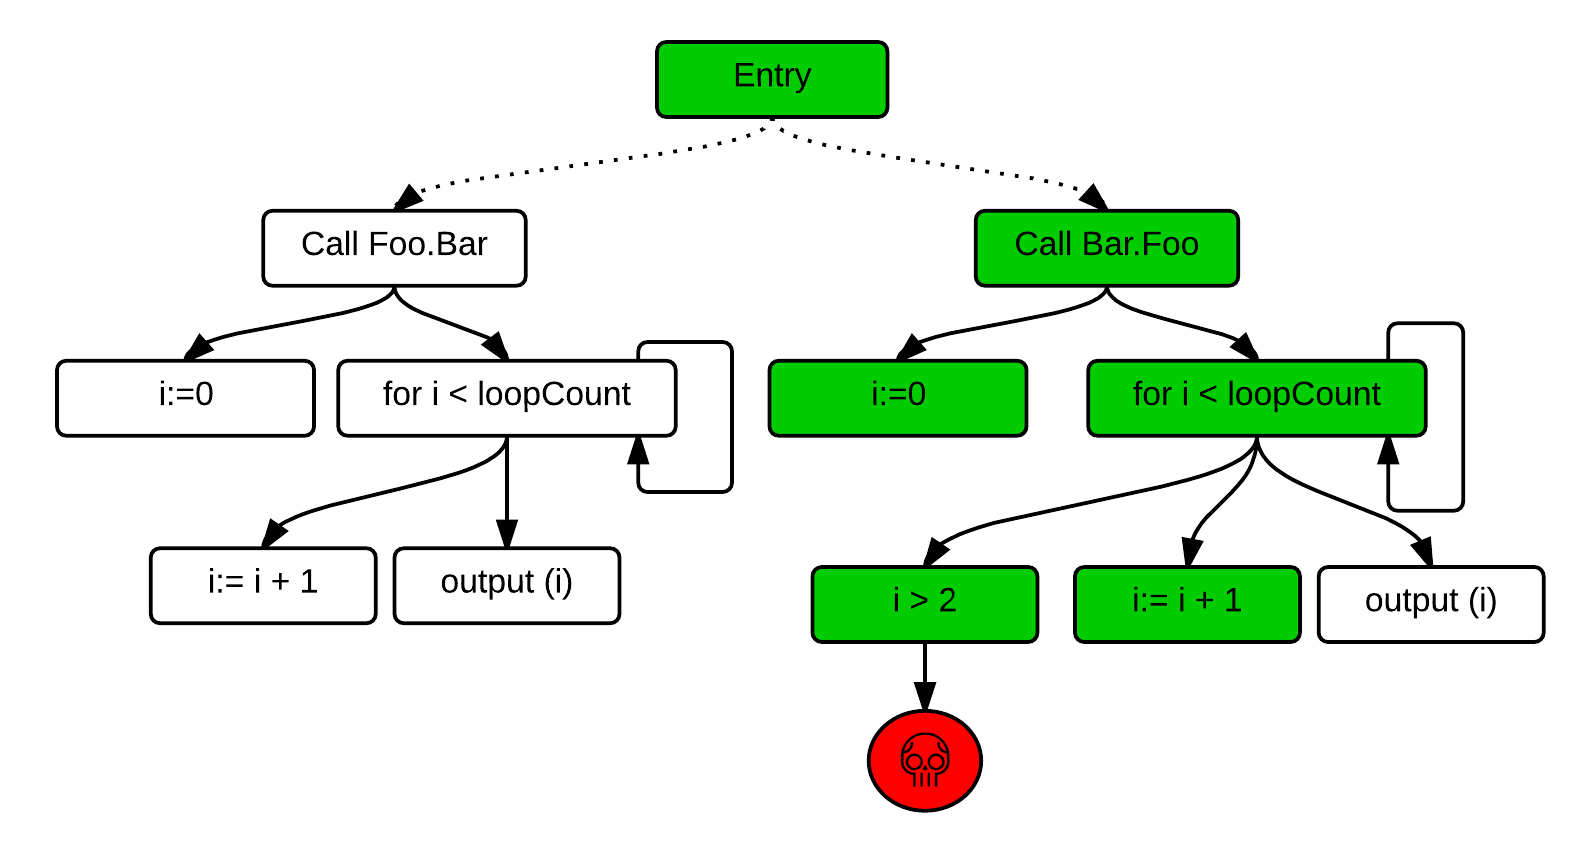
\includegraphics[scale=0.7]{media/dmc.png}
    \caption{A toy program under testing
    \label{fig:testing-toy}}
\end{figure}

\begin{figure}[h!]
  \centering
    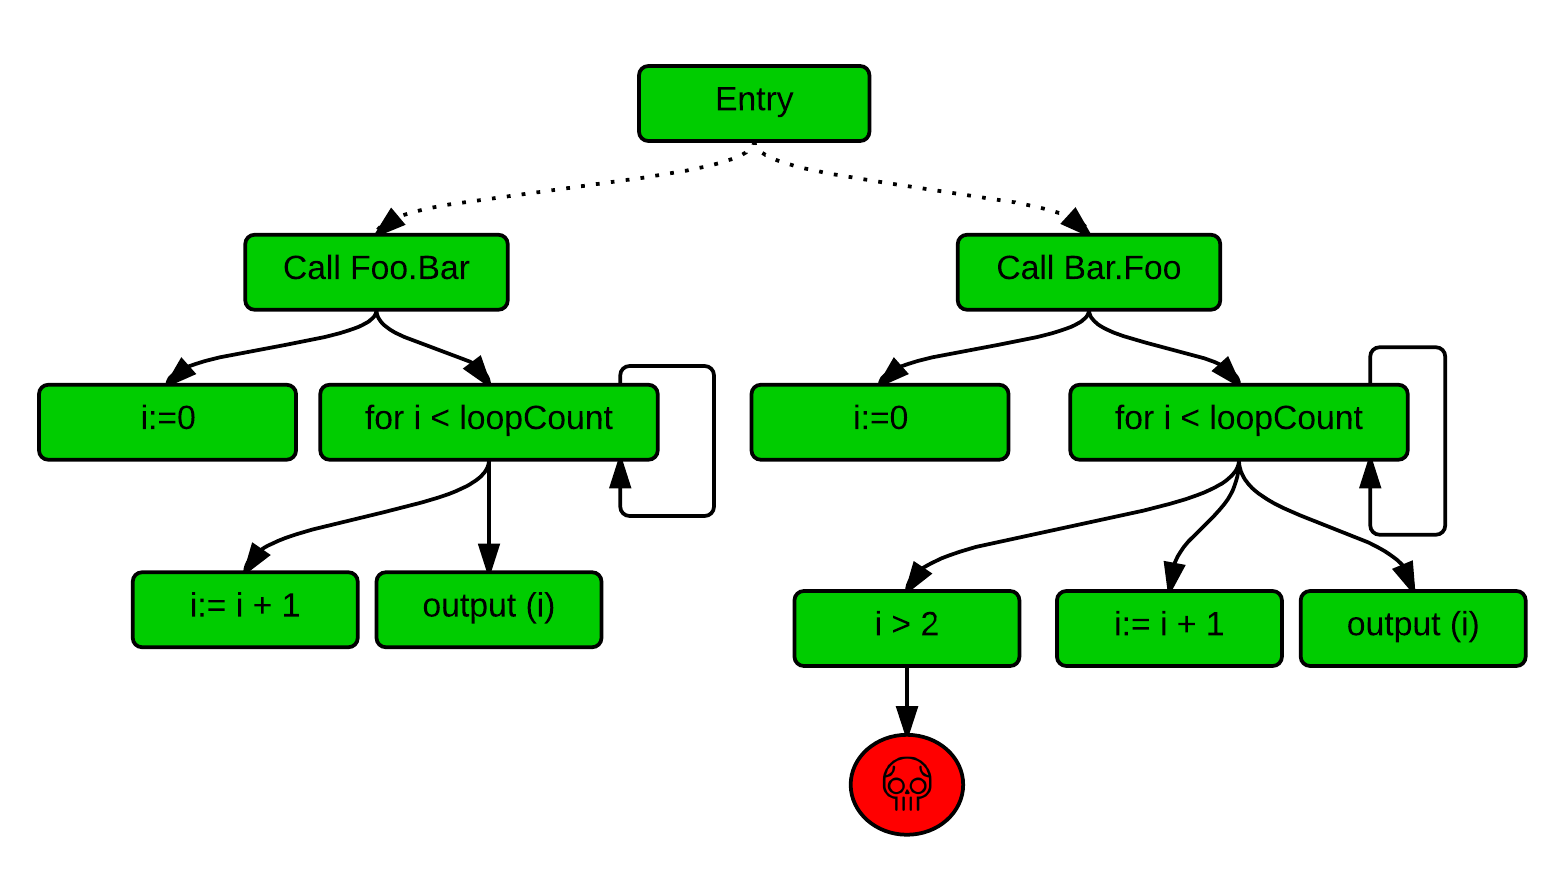
\includegraphics[scale=0.7]{media/mc.png}
    \caption{A toy program under model checking
    \label{fig:checking-toy}}
\end{figure}

\begin{figure}[h!]
  \centering
    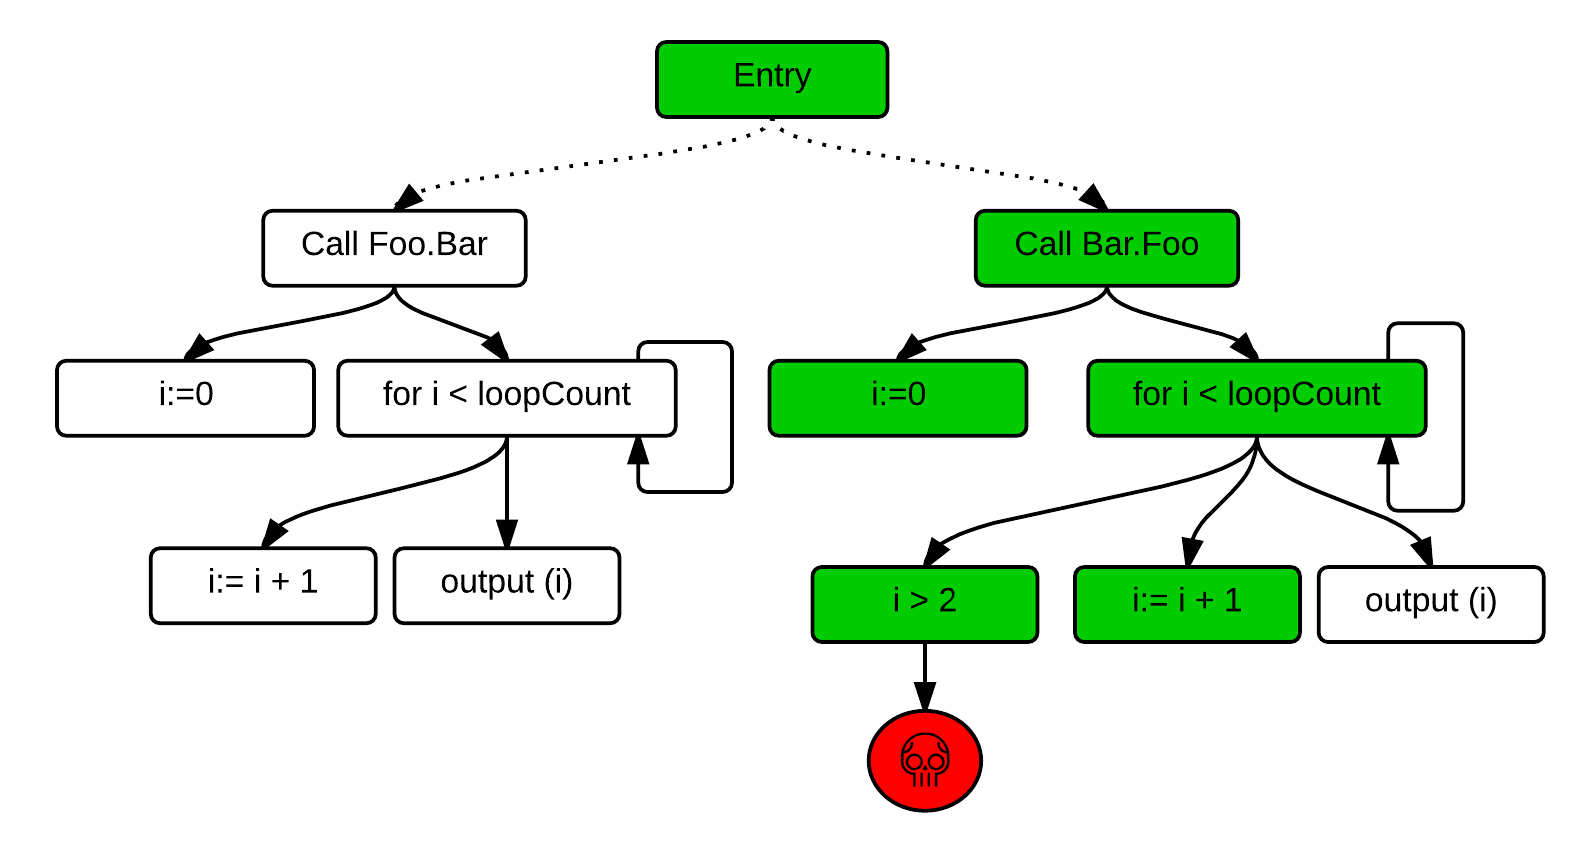
\includegraphics[scale=0.7]{media/dmc.png}
    \caption{A toy program under directed model checking
    \label{fig:dchecking-toy}}
\end{figure}

Figure \ref{fig:testing-toy} shows the program statements that could be covered using testing approaches. Testing software is a demanding task where a set of techniques is used to test the SUT according to some input. Software testing depends on how well the tester understands the SUT in order to write relevant test cases that are likely to find errors in the program. Program testing is usually insufficient because it is not exhaustive. In our case, using testing would mean that the tester knows what to look for in order to detect the causes of the failure. We do not assume this knowledge in JCHARMING.

Model checking, on the other hand, explores each and every state of the program
(Figure \ref{fig:checking-toy}), which makes it complete, but impractical for
real-world and large systems. To overcome the state explosion problem of
model checking, directed (or guided) model checking has been introduced
\cite{Edelkamp2004, Edelkamp2009}. Directed model checking uses insights -- generally
heuristics -- about the SUT in order to reduce the number of states
that need to be examined. Figure \ref{fig:dchecking-toy} explores only
the states that may lead to a specific location, in our case, the
location of the fault. The challenge, however, is to design techniques that
can guide the model checking engine. As we will describe in the next section,
we use crash traces and program slicing to overcome this challenge.

\section{The JCHARMING Approach\label{sec:jcharming}}

Figure \ref{fig:jcarming-approach} shows an overview of JCHARMING. The first step
consists of collecting crash traces (also called stack traces), which contain raw lines
displayed to the standard output when an uncaught exception
in Java occurs. In the second step, the crash traces are
preprocessed by removing noise (mainly calls to Java standard
library methods). \red{The next step is to apply backward slicing
using static analysis to expand the information contained in
the crash trace while reducing the search space. The resulting
slice along with the crash trace is given as input to the model
checking engine.} The model checker executes statements
along the paths from the main function to the first line of the
crash trace (i.e., the last method executed at crash time, also
called the crash location point). Once the model checker finds
inconsistencies in the program leading to a crash, we take the
crash stack generated by the model checker and compare it to
the original crash trace (after preprocessing). The last step is
to build a JUnit test, to be used by software engineers to
reproduce the bug in a deterministic way.

\begin{figure}[h!]
  \centering
    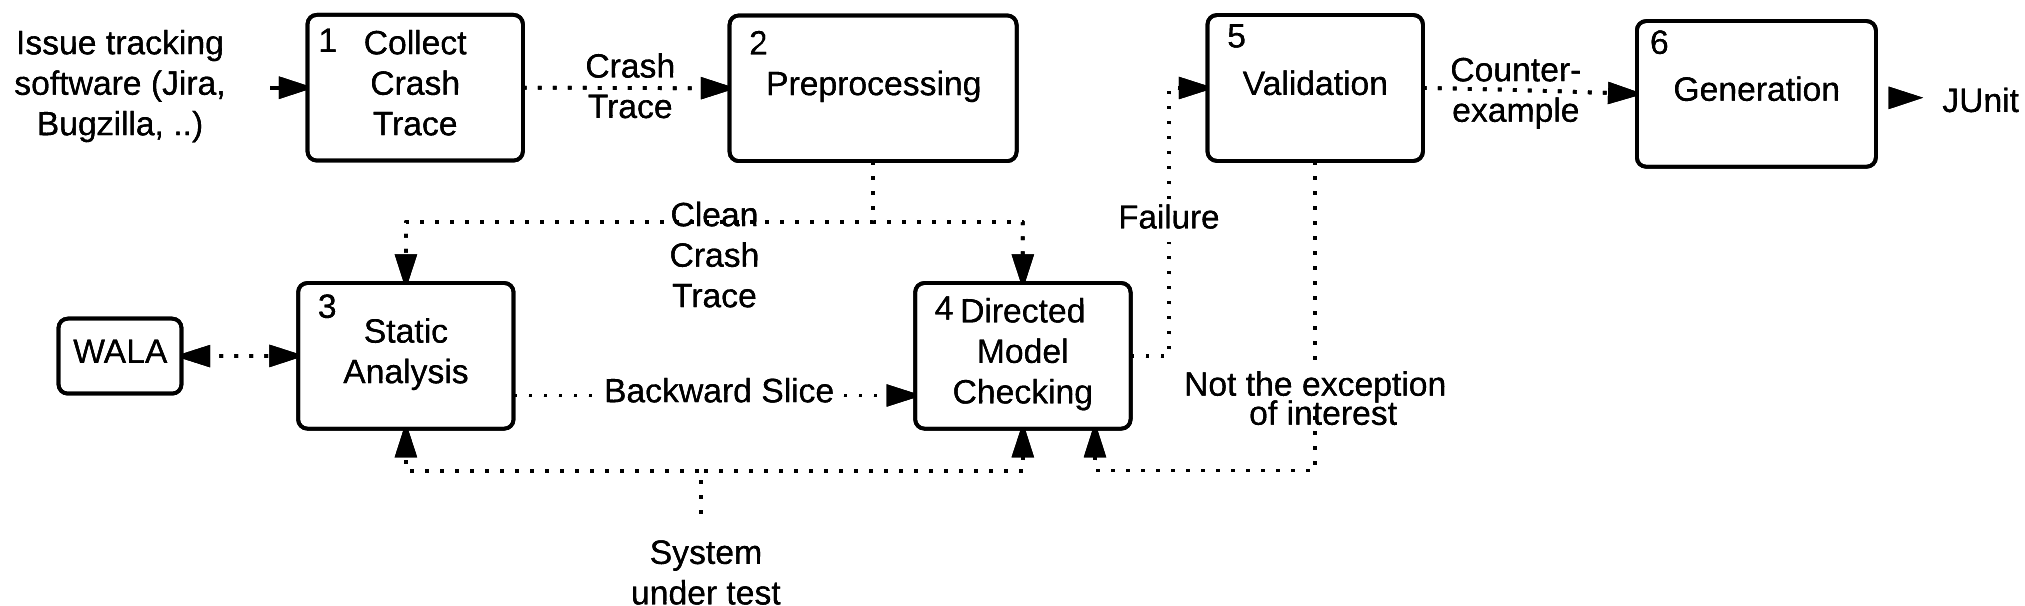
\includegraphics[scale=0.8]{media/jcharming-approach.png}
    \caption{Overview of JCHARMING.
    \label{fig:jcarming-approach}}
\end{figure}

\subsection{Collecting Crash Traces}

The first step of JCHARMING is to collect the crash trace
caused by an uncaught exception. Crash traces are usually included in crash reports and can therefore be automatically
retrieved using a simple regular expression.
Figure \ref{fig:jcarming-traces} shows an example of a crash trace that contains the
exception thrown when executing the program depicted in
Figures \ref{fig:testing-toy} to \ref{fig:dchecking-toy}.
\red{More formally, we define a Java crash trace $T$ of size $N$ as a sequence of frames $T={f_0, f_1, f_2, ..., f_N}$ where each frame represents either a method call and the location of said method, an exception or wrapped exception.
In Figure \ref{fig:jcarming-traces}, the frame $f_0$ represents an exception, the frame  $f_7$ a method call (\texttt{jsep.Foo.buggy}) in a file (\texttt{Foo.java} line 17) leading to the exception and $f_8$ represents a wrapped exception.}

Tt is common in Java to have crash
traces \red{that contain wrapped exceptions.
Such crash traces are incomplete as they do not show all the method calls to go from the entry point of the program to the crash point.}
According to the Java documentation \cite{Oracle2011}, line 8 of
Figure \ref{fig:jcarming-traces} should be interpreted as follows: {\it ``This line indicates
that the remainder of the stack trace for this exception
matches the indicated number of frames from the bottom of the
stack trace of the exception that was caused by this exception
(the ``enclosing exception''). This shorthand can greatly
reduce the length of the output in the common case where a
wrapped exception is thrown from the same method as the
``causative exception'' is caught.}''

We are likely to find shortened traces in bug repositories as
they are what the user sees without any possibility to expand
their content.


\begin{figure}[h!]
  \noindent\fbox{%
      \parbox{\textwidth}{%
  1.javax.activity.InvalidActivityException:loopTimes \\
  should be $<$ 3 \\
  2. at Foo.bar(Foo.java:10) \\
  3. at GUI.buttonActionPerformed(GUI.java:88) \\
  4. at GUI.access\$0(GUI.java:85) \\
  5. at GUI\$1.actionPerformed(GUI.java:57) \\
  6. caused by java.lang.IndexOutOfBoundsException : 3 \\
  7. at jsep.Foo.buggy(Foo.java:17) \\
  8. and 4 more ...
      }%
  }
    \caption{\red{Java InvalidActivityException is thrown in the Bar.Foo loop if the control variable is greater than~2.}
    \label{fig:jcarming-traces}}
\end{figure}


In more details, Figure \ref{fig:jcarming-traces} contains a call to the {\tt Bar.foo()}
method -- the crash location point -- and calls to Java standard
library functions (in this case, GUI methods because the
program was launched using a GUI).
As shown in Figure \ref{fig:jcarming-traces}, we can see that the first line (referred to
as frame {\it $f_0$}, subsequently the next line is called frame {\it $f_1$}, etc.)
does not represent the real crash point but it is only the last
exception of a chain of exceptions. Indeed, the {\tt InvalidActivity}
has been triggered by an {\tt IndexOutOfBoundsException} in
{\tt jsep.Foo.buggy}. This crash trace shows also an example of nested try-catch blocks.



\subsection{Preprocessing}

In the preprocessing step, we first reconstruct and reorganize
the crash trace in order to address the problem of nested
exceptions. Nested exception refers to the following structure in Java. \\

\noindent\fbox{%
  \parbox{\textwidth}{%

1 java.io.IOException: Spill failed \\
... \\
14 Caused by: java.lang.IllegalArgumentException \\
... \\
28 Caused by: java.lang.NullPointerException \\
	}%
 }

\vspace*{0.3cm}

In such a case, we want to reproduce the root exception (line 28)
that led to the other two (lines 14 and 1). This said, we remove the lines
1 to 14.

\red{Then, with the aim to guide the directed model checking engine in an optimal way, we remove frames
that are beyond our control. These refer
to Java library methods and third
party libraries. In Figure \ref{fig:jcarming-traces}, we can see that Java GUI and
event management components appear in the crash trace. We
assume that these methods are not the cause of the crash;
otherwise, it means that there is something wrong with the JDK itself. If this is the case,  we will not be able to reproduce
the crash. Note that removing these unneeded frames will also
reduce the search space of the model checker.}

\subsection{Building the Backward Static Slice}

\red{Static analysis of programs consists of analyzing programs without executing them nor making assumptions about the inputs of the program.
There exist many techniques to perform static analysis (data flow analysis, control flow analysis, theorem proving, ect\ldots) that can be used to improve programs in terms of performances, understandability or to debug them.
One of the products of static analysis is the static slice which takes a program and slicing properties in order to create a smaller program with respect to the slicing properties.
this is particularly interesting for JCHARMING as the sliced program, being smaller, will have a smaller state space.
In Figure \ref{fig:slicing}, black states are states that are impacted by the slicing properties.
After the slicing, the static slice only contains the black states and the states mandatory to reach them.}

\begin{figure}[h!]
  \centering
    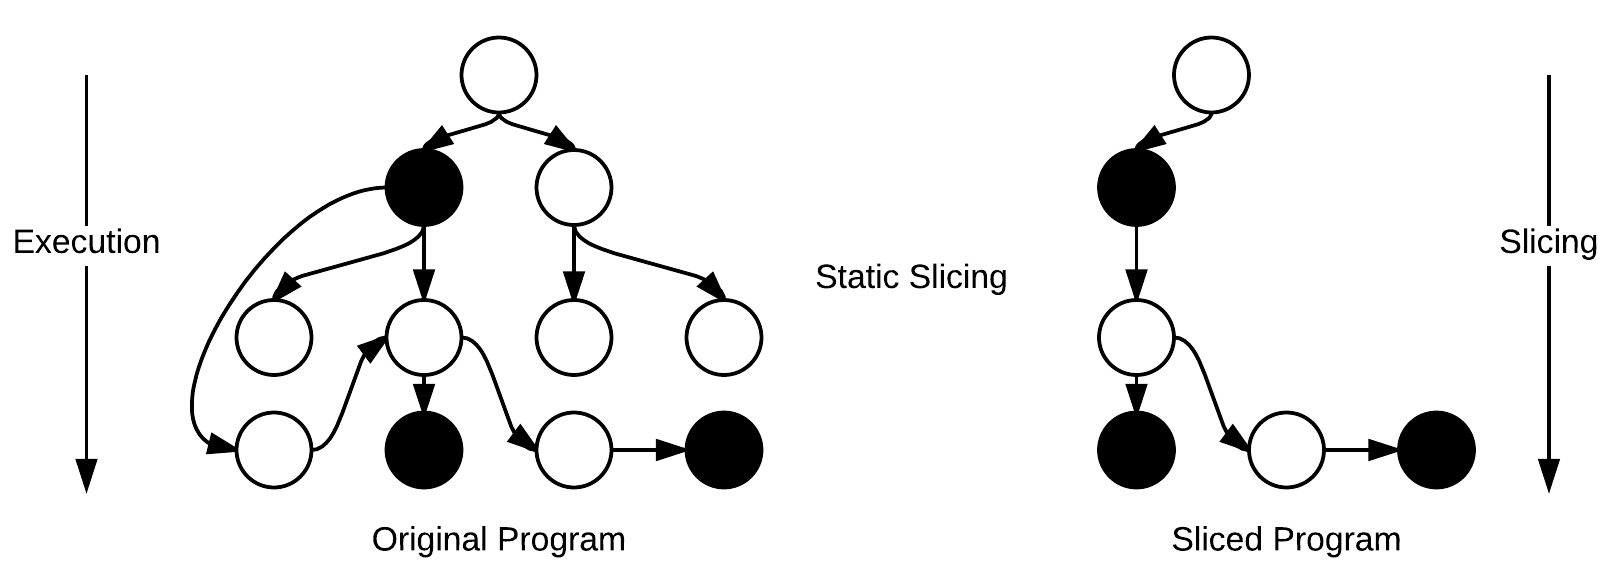
\includegraphics[scale=.25]{media/slicing.png}
    \caption{\red{Hypothetical example of static program slicing}}
    \label{fig:slicing}}
\end{figure}

\red{In JCHARMING, we use a particular static slicing known as backward static slicing.} A backward slice contains all possible branches that may lead
to a point {\it n} from a point {\it m} as well as the definition of the
variables that control these branches \cite{de2001program}. In other words, the
slice of a program point {\it n} is the program subset that may
influence the reachability of point {\it n} starting from point {\it m}.
The backward slice containing the branches and the definition
of the variables leading to {\it n} from {\it m} is noted as {\it $bslice_{[m \leftarrow n]}$}.
\red{Figure \ref{fig:backward-slicing} presents such a backward static slice.}

\begin{figure}[h!]
  \centering
    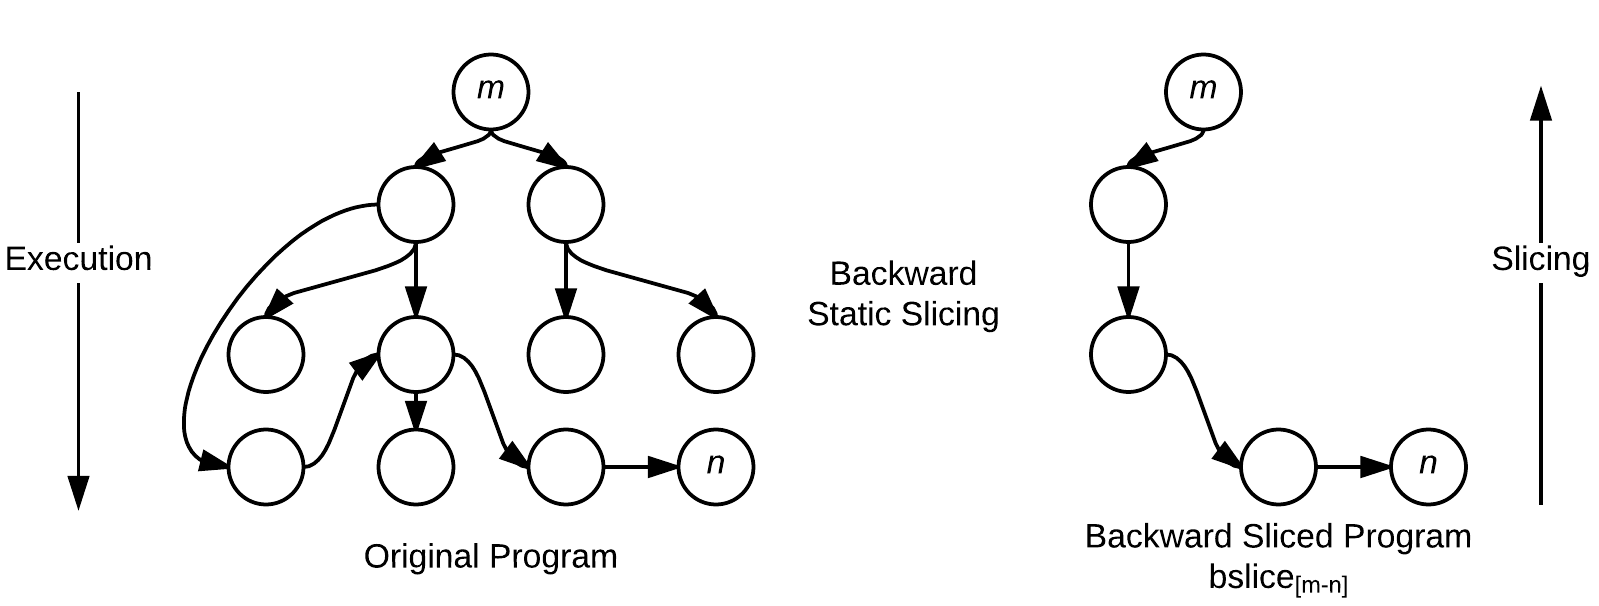
\includegraphics[scale=.25]{media/backward-slicing.png}
    \caption{\red{Hypothetical example of backward static program slicing}}
    \label{fig:backward-slicing}}
\end{figure}


\red{The advantages of computing backward static slice over or static slice are twofold. First, with the stack trace, we have the location of the statement that yields the crash (\textit{n}) and entry point of the program (\textit{m}).} Second, for large systems, a crash trace does not necessarily contain all
the methods that have been executed starting from the entry
point of the program (i.e., the main function) to the crash
location point. We need to complete the content of the crash
trace by identifying all the statements that have been executed
starting from the main function until the last line of the
preprocessed crash trace. In Figure \ref{fig:jcarming-traces}, this will be the function
call \red{{\tt Bar.Foo()}}, which happens to be also the crash location
point. To achieve this, we turn to static analysis by extracting
a backward slice from the main function of the program to the
\red{{\tt Bar.Foo()}} method.

We perform a static backward slice between each frame to
compensate for possible missing information in the crash
trace. More formally, the final static backward slice is
represented as follows:

\begin{equation}
\centering
\begin{split}
bslice_{[entry \leftarrow f_0]} = bslice_{[f_1 \leftarrow f_0]} \cup bslice_{[f_2 \leftarrow f_1]} \cup ... \cup bslice_{[f_n \leftarrow f_{n\−1}]} \cup bslice_{[entry \leftarrow f_n]}
\end{split}
\end{equation}

Note that the union of the slices computed between each pair
of frames must be a subset of the final slice between $f_0$ and the
entry point of the program. More formally:

\begin{equation}
\centering
\begin{split}
\bigcup_{i=0}^{entry-1} bslice_{[f_{i+1} \leftarrow f_i]} \subseteq bslice_{[entry \leftarrow f_0]}
\end{split}
\end{equation}

Indeed, in Figure \ref{fig:jcharming-slice}, the set of states allowing
to reach $f_2$ from
$f_0$ is greater than the set of states to reach $f_2$ from $f_1$ plus set
of states to reach $f_1$ from $f_0$. In this hypothetical example and
assuming that $z_2$ is a prerequisite to $f_2$ then
$bslice_{[entry \leftarrow f_0]} = \{f_0 , f_1 , f_2 , z_0 , z_1 , z_2 , z_3 \}$
while $\cup_{i=0}^n bslice_{[f_{i+1} \leftarrow f_i]}$.

\begin{figure}[h!]
  \centering
    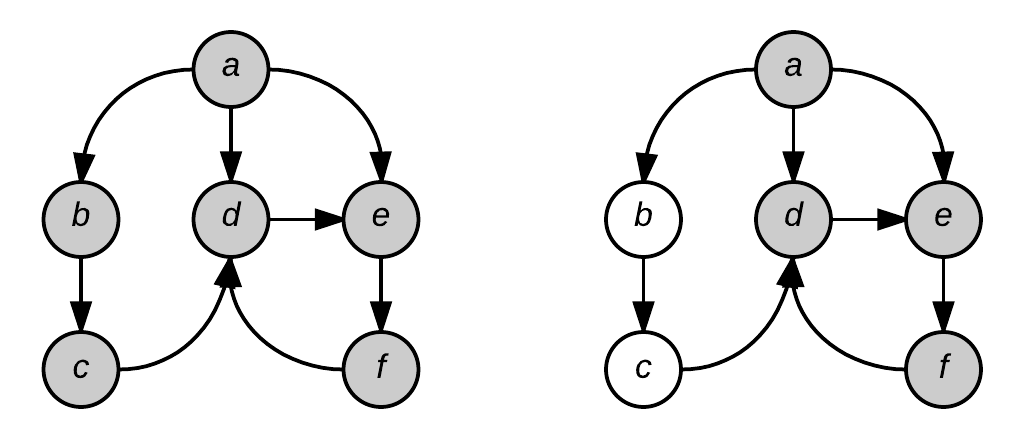
\includegraphics{media/jcharming-slices.png}
    \caption{Hypothetical example representing $bslice_{[entry \leftarrow f_0]}$ Vs. $\cup_{i=0}^n bslice_{[f_{i+1} \leftarrow f_i]} = \{f_0 , f_1 , f_2 , z_2 \}$
    \label{fig:jcharming-slice}}
\end{figure}

\red{In the worst case scenario where there exists one and only one
transition between each two frames (this is very unlikely for real
and complex systems) $bslice_{[entry \leftarrow f_0]}$ and
 $\cup_{i=0}^n bslice_{[f_{i+1} \leftarrow f_i]}$ yield the same set of states with a
comparable computational cost since the number of branches
to explore will be the same in both cases.}


\red{Algorithm \ref{alg:jcharming-slice} is a high-level
representation of how we compute the backward slice between
each frame.
The algorithm takes as input the pre-processed
crash trace $T={f_0, f_1, f_2, ..., f_N}$, the byte code of the SUT, and the entry point. From
line 1 to line 4 we initialize the different variables used by the
algorithm.
Namely, our algorithm needs to have the crash stack as an array of frames (line 1), the size $n$ of the crash stack (line 2) a \texttt{null} backward static slice (line 4) and an offset set to 1 (line 3).
The main loop of the algorithm begins at line 5 and
ends at line 13.
In this loop, we compute the static slice
between the current frame and the next one. If the computed
static slice is not empty then we update the final backward
slice with the newly computed slice.}
If the computed slice is empty, it means that Frame {\tt i + 1}
was corrupted then we move to  Frame {\tt i + 2}, and so on.
At the end of the algorithm, we compute the slice between the
last frame and the entry point of the program, and update the
final slice.

\red{Figure \label{fig:jcharming-algo} presents a step by step graphical reprensentation of Algorithm \ref{alg:jcharming-slice}.
In this figure, an hypothetical program composed of eleven states ($a...k$) crashes in $k$.
The produced stack traces is composed of five frames $T={f_0, f_1, f_2, f_3, f_4, f_5}$.
The frames represents $k$, $i$, $h$, $d$, $b$ and $a$, respectively.
However, $f_3$ has been tampered with and no longer match a location inside the SUT.
In such program, Algorithm \ref{alg:jcharming-slice} will begin by computing the backward static slice between $f_0$ ($k$) and $f_1$ ($i$), then it will compute the backward static slice between  $f_1$ ($i$) and $f_2$ ($h$).
At this point, we passed through the $for$ loop (line 5 to 12) two times and both times, the backward static slice was not empty.
Consequently, the $if$ statement was equal to $true$ and we combined both backward static slice in the $bSlice$ variable.
$bSlice$ is equal to \{$k$, $j$, $i$, $h$\}.
Then, we want to compute the backward static slice between $f_2$ ($h$) and $f_3$ ($d$).
Unfortunately, $f_3$ is corrupted and do not point towards a valid location in the SUT.
The corruption can be the result of a copy-pasting error or a deliberate intervention of the reported as shown in Section \ref{sec:results}.
Consequently, the backward static slice between $f_2$ ($h$) and $f_3$ ($d$) will be empty, and we will go to the $else$ statement (line 10).
Here, we simply increment $offset$ by one in order to compute the backward static slice from $f_2$ ($h$) and $f_4$ ($b$) instead of $f_2$ ($h$) and $f_3$ ($d$).
$f_4$ is not corrupted and the backward static slice from $f_2$ ($h$) and $f_4$ ($b$) can be computed and merged to $bSlice$.
Finally, we compute the last slice between $f_4$ ($b$) and $f_5$ ($a$).
The final backward static slice is $k$, $i$, $h$, $d$, $b$ and $a$.}

\vspace*{0.3cm}

\begin{algorithm}[H]
 \KwData{Crash Stack, BCode, Entry Point}
 \KwResult{BSolve}
 Frame[]~frames $\leftarrow$ extract~frames~from~crash~stack; \\
 Int n $\leftarrow$ size of frames\;
 Int offset $\leftarrow$ 1\;
 Bslice bSlice $\leftarrow$ $\emptyset$\;
\For{i $\leftarrow$ 0; (i $<$ n \&\& offset $<$ n - 1); i++}{
  BSlice currentBSlice $\leftarrow$ backward slice from frames[i] to frames[i + offset]\;
  \eIf{currentBSlice $\not=$ $\emptyset$}{
   bSlice $\leftarrow$ bSlice $\cup$ currentBSlice\;
   offset $\leftarrow$ 1\;
  }{
   offset $\leftarrow$ offset +1\;
  }
}
\caption{High level algorithm computing the union of the slices\label{alg:jcharming-slice}}
\end{algorithm}

\vspace*{0.3cm}


\begin{figure}[h!]
  \centering
    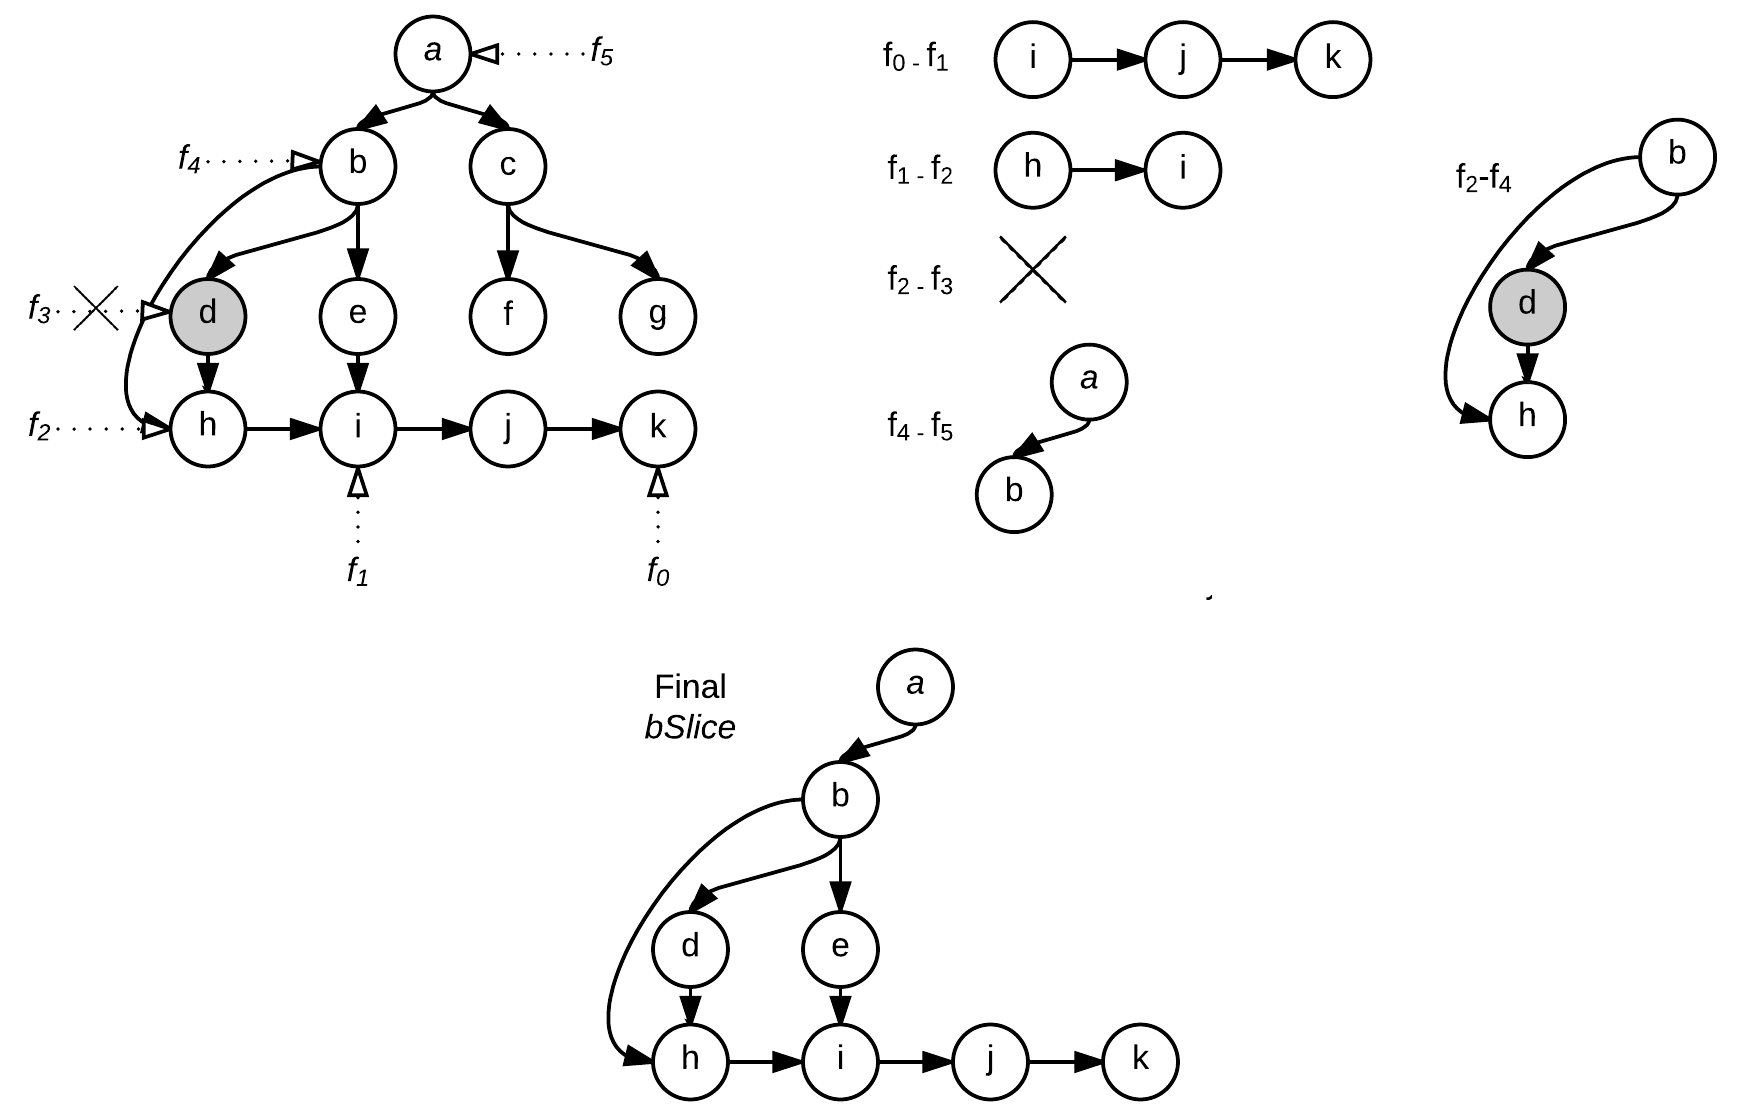
\includegraphics[scale=.20]{media/algo.png}
    \caption{\red{Steps of Algorithm \ref{alg:jcharming-slice} where $f_3$ is corrupted.}
    \label{fig:jcharming-algo}}
\end{figure}

\red{Our algorithm, given an uncorrupted stack trace will be able to compute an optimum backward static slice based on the frames (Figure~\ref{fig:jcharming-slice}) and compensate for frames corruption if needs be by \texttt{offsetting} the corrupted frame (Figure~\ref{fig:jcharming-algo}).
The compensation of corrupted frames, obviously, comes at the cost of a sub-optimum backward static slice.
In our previous example, the transition between $b$ and $h$ could have been omitted if $f_3$ was not corrupted.
}


\red{In the rare cases where the final slice is empty (this
may happen in situations where the content of the crash trace
is seriously corrupted) JCHARMING would simply
proceed with non-directed model checking.}




Note that while we allow in JCHARMING the possibility to resort to non-directed
model
checking, none of the 30 bugs used in this study contained crash traces
that were damaged enough for this fall back mechanism to be used.

\red{In order to compute the backward slice, we implement our
algorithm as an add-on to the T. J. Watson
Libraries for Analysis (WALA)\cite{IBM2006}, which provide static
analysis capabilities for Java Bytecode and JavaScript.}  WALA offers a very comprehensive API
to perform static backward slicing on Java Bytecode from a
specific point to another.
We did not need to extend WALA to perform our
analysis.

At first sight, it may appear that static slicing alone can be
used to reproduce the bug since it contains all the functions
that lead to the first user-defined method of the crash trace.
The problem is that a static slice may also contain many other
parts of the program that are not relevant to the failure. A
quick solution to this is to prune out the content of the
resulting static slice by eliminating the unwanted statements.
This can be achieved by defining specific inputs. The result
will be a dynamic slice. This assumes that we know in
advance which input we need to provide to the program in
order to reach the crash, which defeats the purpose of bug
reproduction in the first place. \\


Using backward slicing, the search space of the model checker
that processes the example of Figures \ref{fig:testing-toy} to \ref{fig:dchecking-toy} is given by the
following expression:

\begin{equation}
  \exists x.
  \begin{pmatrix}
    \bigcup_{i=0}^{entry} bslice_{[f_{i+1} \leftarrow f_i]}  \subset SUT, \\
    x.\bigcup_{i=0}^{entry} bslice_{[f_{i+1} \leftarrow f_i]}  \subset x.SUT
  \end{pmatrix}
  \models c_{i>2}
\end{equation}

That is, there exists a sequence of state transitions $x$ that
satisfies $c_{i>2}$ where both the transitions and the states are
entry
elements of $\bigcup_{i=0}^{entry} bslice_{[f_{i+1} \leftarrow f_i]}$ . Obviously, $c_{i>2}$ also
needs to be included for the final static slice to be usable by
the model checking engine. \red{That is, the only frame that
needs to be untouched for the backward static slice to be
meaningful is $f_0$.
If the first line of the stack trace, i.e., frame 0, is corrupt then JCHARMING cannot perform the slicing because  it does not know where to go. The result is a non-directed model checking which is likely to fail.}

\subsection{Directed Model Checking}

The model checking engine we use in this paper is called JPF
(Java PathFinder) \cite{Visser2004}, which is an extensible JVM for Java
bytecode verification. This tool was first created as a front-end
for the SPIN model checker \cite{holzmann1997model} in 1999 before being
open-sourced in 2005.
\red{The JPF model checker can execute all the bytecode instructions
and, therefore, allow the whole Java language to be model checked. Its consists of a custom JVM --- known as JVM\textsuperscript{\textit{JPF}} --- that executes the bytecode instructions.
This custom JVM supports all the existing Java bytecode instructions and, therefore, is able to execute any \textit{pure}\footnote{In opposition to a Java program with native call.} java programs.
Furthermore, JPF is an explicit state model checker
very much like SPIN \cite{holzmann1997model} and not a symbolic model
checker based on binary decision diagrams \cite{mcmillan1993symbolic}.
JPF designers opted for a a depth-first traversal with backtracking
as they thought it will be superior to breadth-first for checking for checking temporal liveness properties.
Currently\footnote{JPF is still under development at the NASA Babelfish lab.}, the JPF model checker is able to check deadlocks, invariants, and user-defined code assertion as same as LTL (Linear Time Logic) properties.}

JPF is organized around five simple
operations: (i) {\it generate states}, (ii) {\it forward}, (iii) {\it backtrack},
(iv) {\it restore state} and (v) {\it check}.
In the forward operation, the
model checking engine generates the next state $s_{t+1}$.
\red{Each state consists of three distinct component: }
\begin{itemize}
  \item \red{The information of each thread. More specifically, a stack of frames corresponding to methods' calls.}
  \item \red{The static variables of a given class.}
  \item \red{The dynamic variables of a given object.}
\end{itemize}
If $s_{t+1}$ has successors then it is saved in a backtrack table to be
restored later. \red{The backtrack operation consists of restoring
the last state in the backtrack table. The restore operation
allows restoring any state. It can also be used to restore the entire
program as it was the last time we chose between two
branches.} After each, forward, backtrack and restore state
operation the check properties operation is triggered.

In order to direct JPF, we have to modify the {\it generate states}
and the {\it forward} steps. The {\it generate states} is populated with
the states in $\bigcup_{i=0}^{entry} bslice_{[f_{i+1} \leftarrow f_i]}  \subset SUT$ and we adjust the
{\it forward step} to explore a state if the target state $s_i+1$ and the
transition $x$ to pass from the current state $s_i$ to $s_{i+1}$ are in
$\bigcup_{i=0}^{entry} bslice_{[f_{i+1} \leftarrow f_i]}  \subset SUT$ and $x.\bigcup_{i=0}^{entry} bslice_{[f_{i+1} \leftarrow f_i]}  \subset x.SUT$.

In other words, JPF does not generate each possible state for the system under test.
Instead, JPF generates and explores only the states that fall inside the backward static
slice we computed in the previous step.
As shown in figure \ref{fig:jcharming-slice}, our backward static slice can
greatly reduces the space search and is able to compensate for corrupted frames.
In short, the idea is that instead of going through all the states of the program as a
complete model checker would do, the backward slice directs the model checker to explore
only the states that might reach the targeted frame.

\subsection{Validation}

\red{To validate the result of directed model checking, we modify
the {\it check properties} step that checks if the current sequence
of state transition $x$ satisfies a set of properties. If the current
state transition $x$ can throw an exception, we execute $x$ and
compare the exception thrown to the original crash trace (after
preprocessing). If the two exceptions match, we conclude that
the conditions needed to trigger the failure have been met and
the bug is reproduced.}

However, as argued by Kim {\it et al.} in \cite{Kim2013b}, the same failure can
be reached from different paths of the program. Although the
states executed to reach the defect are not exactly the same,
they might be useful to enhance the understanding of the bug
by software developers, and speed up the deployment of a fix.
Therefore, in this paper, we consider a defect to be partially
reproduced if the crash trace generated from the model
checker matches the original crash trace by a factor of $t$, where
$t$ is a threshold specified by the user. \red{Thus, $t$ is the percentage of
identical frames between both crash traces.}

For our experiments (see Section \ref{sec:results}), we set the value of $t$ to 80\%.
The choice of $t$ should be guided by the need to find the best trade-off
between the reproducibility of the bug and
the relevance  of the generated test cases (the tests should help
 reproduce the on-field crash). To determine the best $t$, we made several incremental attempts, starting  from $t = 10\%$.  For each attempt, we increased $t$ with a factor of 5\% and
observed the number of bugs reproduced and the quality of the generated tests.
\red{Having $t = 80\%$ provided the best trade-off. This said, we anticipate that the tool that implements
our technique should allow software engineers to vary $t$ depending on the bugs and the systems under study. Based on our observations, we recommend, however,
to set $t$ to 80\% as a baseline. It should also be noted that we deliberately prevented JCHARMING to perform directed model checking with a threshold below 50\%. This is because the tests generated with such a low threshold during our experiments did not yield qualitative results.}


\subsection{Generating Test Cases for Bug Reproduction}

\red{To help software developers reproduce the crash in a lab
environment, we automatically produce the JUnit test cases
necessary to run the SUT to cause the bug to appear.}

To build a test suite that reproduces a defect, we need to create
a set of objects used as arguments for the methods that will
enable us to travel from the entry point of the program to the
defect location. JPF has the ability to keep track of what
happens during model checking in the form of traces
containing the visited states and the value of the variables. We
leverage this capability to create the required objects and call
the methods leading to the failure location.

\red{During the testing of the SUT, JPF emits a trace that is composed of the executed instructions.
For large systems, this trace can contain millions of instructions. This trace is stored in memory and therefore can be queried while JPF is running.
However, accessing the trace during the JPF execution considerably slows down the checking process as both the querying mechanism and the JPF engine compete with each other for resources.
In order to allow JPF to use 100\% of the available resources and still be able to query the executed instructions, we implemented a {\tt listener} that listens to the JPF trace emitter.
Each time a new instruction is processed by JPF, our listener catches it and then saves it to a MongoDB database to be queried in a post-mortem fashion. Figure \ref{fig:jcharming-unittest} presents a high-level architecture of the components of the JUnit test generation process.}

\begin{figure}[h!]
  \centering
    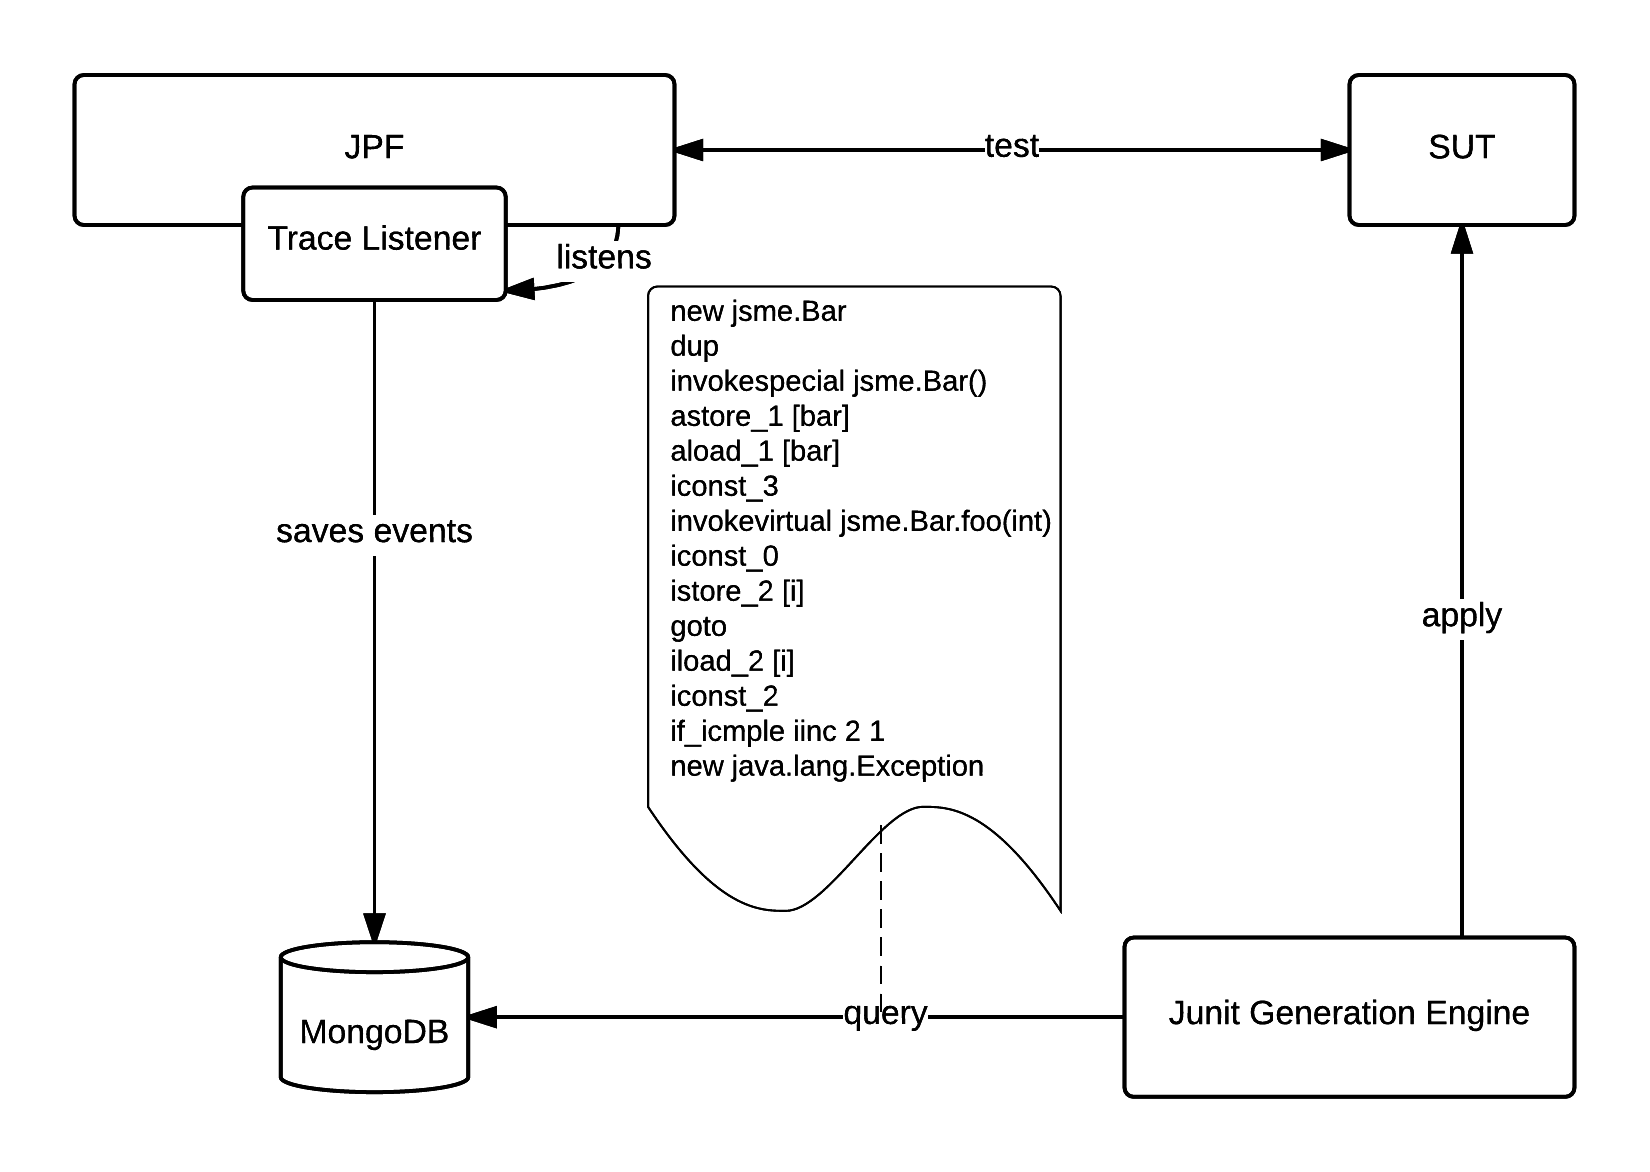
\includegraphics[scale=0.8]{media/unittest.png}
    \caption{High level architecture of the Junit test case generation
    \label{fig:jcharming-unittest}}
\end{figure}


When the {\tt validate} step triggers a crash stack with a similarity larger than a factor {\tt t}, the JUnit generation engine queries the MongoDB database and fetches the sequence of instructions that led to the crash of interest.
Figure \ref{fig:jcharming-unittest} contains a hypothetical sequence
of instructions related to the example of Figures \ref{fig:testing-toy},
\ref{fig:checking-toy}, \ref{fig:dchecking-toy}, which reads : {\tt new jsme.Bar},
 {\tt invokespecial jsme.Bar()}, {\tt astore\_1 [bar]}, {\tt aload\_1 [bar]},
  {\tt iconst\_3}, {\tt invokevirtual jsme.Bar.foo(int)}, {\tt const\_0},
  {\tt istore\_2 [i]}, {\tt goto}, {\tt iload\_2 [i]}, {\tt iconst\_2},
  {\tt if\_icmple iinc 2 1}, {\tt new java.lang.Exception}.
From this sequence we know that, to reproduce to crash of interest, we have
to (1) create a new object {\tt jsme.Bar} ({\tt new jsme.Bar},
{\tt invokespecial jsme.Bar()}), (2) store the newly created object in a
variable named {\tt bar} ({\tt astore\_1 [bar]}), (3) invoke the method
{\tt jsme.Bar.foo(int)} of the {\tt bar} object with {\tt 3} as value
({\tt aload\_1 [bar]}, {\tt iconst\_3}, {\tt invokevirtual jsme.Bar.foo(int)}).
Then, the {\tt jsme.Bar.foo(int)} method will execute a $for-loop$ from $i=0$ until $i=3$ and
throw an exception at {\tt i = 3}~({\tt const\_0}, {\tt istore\_2 [i]}, {\tt goto},
{\tt iload\_2 [i]}, {\tt iconst\_2}, {\tt if\_icmple iinc 2 1}, {\tt new java.lang.Exception}).

\red{The generation of the JUnit test itself is based on templates and targets directly
the system under test. Templates are excerpts of Java source code with well-defined
tags that will be replaced by values. We use templates because the
JUnit test cases have common structures.
Figure \ref{fig:jcharming-unittemplate} shows our template for generating JUnit
test cases. In this figure, each {\tt \{\% \%\}} will be dynamically replaced by
the corresponding value when the JUnit test is generated. For example, {\tt \{\% SUT \%\}}
will be replaced by {\tt Ant} if the SUT is Ant.
First, we declare four variables that contain the {\tt failure},
the {\tt threshold} above which a given bug is said to be partially reproduced,
the {\tt differences} which count how many lines differ between the original
failure and the failure produced by JCHARMING and a {\tt StringTokenizer}.
The {\tt StringTokenizer} allows to break the original {\tt failure} into
tokens. Second, the test method where {\tt \{\%SUT\%\}} is replaced by the name
of the SUT and {\tt \{\%STEPS\%\}} by the steps to make the SUT crash.
Then, the stack trace related to the crash is received in the {\tt catch} part of
the {\tt try-catch} block. In the {\tt catch} part, we compute the number of lines
that do not match the original exception and store it into {\tt differences}
\footnote{This code has been replaced by {\tt //Count the differences} to ease the
reading.}.Finally, the {\tt assertTrue} call will assert that
the crash traces from the induced and the original crash are at least {\tt threshold}
 percent similar to each other.}


\begin{figure}[h!]

\noindent\fbox{%
    \parbox{\textwidth}{%
    \lstinputlisting[language=Java]{test.java}
}%
}

    \caption{Simplified Unit Test template
    \label{fig:jcharming-unittemplate}}
\end{figure}

\section{Case studies\label{sec:cases}}

In this section, we show the effectiveness of JCHARMING to
reproduce bugs in ten open source systems
\footnote{\red{The bug reports used in this study and the result of JCHARMING are
made available for download from https://research.mathieu\-nayrolles.com/jcharming/}}. The aim of the
case studies is to answer the following question: {\it Can we use
crash traces and directed model checking to reproduce on-
field bugs in a reasonable amount of time?}

\subsection{Targeted Systems}

Table \ref{tab:jacharming-systems} shows the systems and their characteristics in terms of
Kilo Line of Code (KLoC) and Number of Classes (NoC).

\begin{table}[h!]
\centering

\caption{List of target systems in terms of Kilo line of code (KLoC), number of classes (NoC) and Bug \# ID}
\begin{tabular}{c|c|c|c}
SUT        & KLOC & NoC  & Bug \#ID                                        \\ \hline \hline
Ant        & 265  & 1,233 & 38622, 41422                                    \\
ArgoUML    & 58   & 1,922 & 2603, 2558, 311, 1786                           \\
dnsjava    & 33   & 182  & 38                                              \\
jfreechart & 310  & 990  & 434, 664, 916                                   \\
Log4j      & 70   & 363  & 11570, 40212, 41186, 45335, 46271, 47912, 47957 \\
MCT        & 203  & 1267 & 440ed48                                         \\
pdfbox     & 201  & 957  & 1,412, 1,359 \\
\red{Hadoop} 	   & 308   & 6,337 & 2893, 3093, 11878\\
\red{Mahout} 	   & 287  & 1,242 &  486, 1367, 1594, 1635\\
ActiveMQ   & 205  & 3,797 & 1054, 2880, 2880\\ \hline
Total      & 1,517 & 17,348 & 30 \\
\hline \hline
\end{tabular}
\label{tab:jacharming-systems}
\end{table}


\red{Apache Ant \cite{ApacheSoftwareFoundation} is a popular command-line tool to build
Makefiles.} While it is mainly known for Java applications,
Apache Ant also allows building C and C++ applications. We
choose to analyze Apache Ant because it has been used by
other researchers in similar studies.

\red{ArgoUML \cite{CollabNet} is one of the major players among the open source
UML modeling tools.} It has many years of bug management
and, similar to Apache Ant, it has been extensively used as a
test subject in many studies.

Dnsjava \cite{Wellington2013} is a tool for the implementation of the DNS
mechanisms in Java. This tool can be used for queries, zone
transfers, and dynamic updates. It is not as large as the other
two, but it still makes an interesting case subject because it has
been well maintained for the past decade. Also, this tool is
used in many other popular tools such as Aspirin, Muffin and
Scarab.

JfreeChart \cite{ObjectRefineryLimited2005} is a well-known library that enables the
creation of professional charts. \red{Similar to dnsjava, it has been
maintained over a very long period of time. JfreeChart was
created in 2005. It is a relatively large application.}

Apache Log4j \cite{TheApacheSoftwareFoundation1999} is a logging library for Java.
This is not a
very large library, but it is extensively used by thousands of
programs. As other Apache projects, this tool is well
maintained by a strong open source community and allows
developers to submit bugs. The bugs that are in the bug
reporting system of Log4j are generally well
documented. In addition, the majority of bugs contain crash
traces, which makes Log4j a good candidate system for this study.

MCT \cite{NASA2009} stands for Mission Control technologies and was
developed by the NASA Ames Research Center (the creators
of JPF) for use in spaceflight mission operation. This tool
benefits from two years of history and targets a very critical
domain, Spacial Mission Control. Therefore, this tool has to
be particularly and carefully tested and, consequently, the
remaining bugs should be hard to discover and reproduce.

PDFBox \cite{ApacheSoftwareFoundation2014} is another tool supported by the Apache
Software Foundation since 2009 and was created in 2008.
PDFBox allows the creation of new PDF documents and the
manipulation of existing documents.

Hadoop \cite{hadoop2011hadoop} is a framework for storing and processing large datasets in a distributed environment. It contains four main modules: {\it Common}, {\it HDFS}, {\it YARN} and {\it MapReduce}. In this paper, we study the {\it Common} module that contains the different libraries required by the other three modules.

Mahout \cite{mahout2012scalable} is a relatively new software application, built on top of Hadoop. \red{We used Mahout version 0.11, which was released in August 2015.}
Mahout supports various machine learning algorithms with a focus on collaborative filtering, clustering, and classification.

Finally, ActiveMQ \cite{snyder2011activemq} is an open source messaging server that allows applications written in Java, C, C++, C\#, Ruby, Perl or PHP to exchange messages using various protocols. ActiveMQ has  been actively maintained since it became an Apache Software Foundation project in 2005.


\pagebreak

\vspace*{3cm}

\begin{table}[h!]
\centering
\caption{Effectiveness of JCHARMING using directed model checking (DMC) and model checking (MC) in minutes}
\begin{tabular}{c|c|c|c|c}
SUT                         & Bug \#ID & Reprod. & Time DMC & Time MC \\ \hline \hline
\multirow{2}{*}{Ant}        & 38622    & Yes     & 25.4     & -       \\
                            & 41422    & No      & 42.3     & -       \\ \hline
\multirow{4}{*}{ArgoUML}    & 2558     & Partial & 10.6     & -       \\
                            & 2603     & Partial & 9.4      & -       \\
                            & 311      & Yes     & 11.3     & -       \\
                            & 1786     & Partial & 9.9      & -       \\  \hline
DnsJava                     & 38       & Yes     & 4        & 23      \\ \hline
\multirow{3}{*}{jFreeChart} & 434      & Yes     & 27.3     & -       \\
                            & 664      & Partial & 31.2     & -       \\
                            & 916      & Yes     & 26.4     & -       \\ \hline
\multirow{7}{*}{Log4j}      & 11570    & Yes     & 12.1     & -       \\
                            & 40212    & Yes     & 15.8     & -       \\
                            & 41186    & Partial & 16.7     & -       \\
                            & 45335    & No      & 3.2      & -       \\
                            & 46271    & Yes     & 13.9     & -       \\
                            & 47912    & Yes     & 12.3     & -       \\
                            & 47957    & No      & 2        & -       \\ \hline
MCT                         & 440ed48  & Yes     & 18.6     & -       \\ \hline
\multirow{2}{*}{PDFBox}     & 1412     & Partial & 19.7     & -       \\
                            & 1359     & No      & 7.5        & - \\ \hline
\multirow{4}{*}{Mahout}   & 486      & Partial & 34.5     & -        \\
                            & 1367     & Partial & 21.1     & -       \\
                            & 1594 	   & No 	 & 14.8 	    & -       \\
                            & 1635     & Yes     & 31.0     & - \\ \hline
\multirow{3}{*}{Hadoop}     & 2893     & Partial & 7.4      & 32       \\
						    & 3093     & Yes 	 & 13.1     & -        \\
                            & 11878    & Yes 	 & 17.4     & - \\  \hline
\multirow{3}{*}{ActiveMQ}   & 1054     & Yes     & 38.3     & -      \\
						    & 2880     & Partial & 27.4        & -        \\
                            & 5035     & No 	 & 1    & - \\  \hline \hline
\end{tabular}


\label{tab:jcharming-results}
\end{table}

\pagebreak

\subsection{Bug Selection and Crash Traces}

In this study, we have selected the reproduced bugs randomly
in order to avoid the introduction of any bias. We selected a
random number of bugs ranging from 1 to 10 for each SUT containing the word ``exception'' and where the description of
the bug contains a match to a regular expression designed to find the pattern of a
Java exception.

\section{Results\label{sec:results}}

Table \ref{tab:jcharming-results} shows the results of JCHARMING in terms of Bug
\#ID, reproduction status, and execution time (in minutes) of
directed model checking (DMC) and Model Checking (MC).
The experiments have been conducted on a Linux machine (8
GB of RAM and using Java 1.7.0\_51).

\begin{itemize}
  \item The result is noted as ``Yes'' if the bug has been fully
reproduced, meaning that the crash trace generated by the
model checker is identical to the crash trace collected
during the failure of the system.
\item \red{The result is ``Partial'' if the similarity between the crash
trace generated by the model checker and the original
crash trace is above t=80\% and below t=100\%. Given an 80\% similarity
threshold, we consider partial reproduction as successful.
A different threshold could be used.}
\item Finally, the result of the approach is reported as ``No'' if
either the similarity is below $t < 80\%$ or the model
checker failed to crash the system given the input we
provided.
\end{itemize}


\red{As we can see in Table \ref{tab:jcharming-results}, we were able to reproduce 24 bugs
out of 30 bugs either completely or partially (80\% success ratio). The average time to reproduce a bug was 19 minutes. The average time in cases where JCHARMING failed to reproduce the bug  was 11 minutes. The maximum fail time was 42.3 minutes, which was the time
required for JCHARMING to fill all the available memory and stop. Finally, a ``-'' denotes that JCHARMING reached a 60 minutes timeout.
This result demonstrates the effectiveness of our approach,
more particularly, the use of backward slicing to create a
manageable search space that guides adequately the model
checking engine.} We also demonstrated that our approach is usable
in practice since it is also time efficient. Among the 30 different bugs we have tested, we will describe
two bugs (chosen randomly) for each category (successfully
reproduced, partially reproduced, and not reproduced) for
further analysis.
\red{The bug report presented in the following sections are the original reports as submitted by the reporter.
As such, they contain typos and spelling mistakes that we did not correct.}

\subsection{Successfully Reproduced}

The first bug we describe in this discussion is the bug \#311
belonging to ArgoUML. This bug was submitted in an earlier
version of ArgoUML. This bug is very simple to manually
reproduce thanks to the extensive description provided by the
reporter, which reads: {\it ``I open my first project (Untitled Model by default). I choose
to draw a Class Diagram. I add a class to the diagram. The
class name appears in the left browser panel. I can select the
class by clicking on its name. I add an instance variable to the
class. The attribute name appears in the left browser panel. I
can't select the attribute by clicking on its name. Exception
occurred during event dispatching:''}



The reporter also attached the following crash trace that we
used as input for JCHARMING:

\vspace*{0.3cm}

\noindent\fbox{%
    \parbox{\textwidth}{%
1. java.lang.NullPointerException:\\
2. at\\
3. uci.uml.ui.props.PropPanelAttribute
.setTargetInternal (PropPanelAttribute.java)\\
4. at uci.uml.ui.props.PropPanel.
setTarget(PropPanel.java)\\
5. at uci.uml.ui.TabProps.setTarget(TabProps.java)\\
6. at uci.uml.ui.DetailsPane.setTarget
(DetailsPane.java)\\
7. at uci.uml.ui.ProjectBrowser.select
(ProjectBrowser.java)\\
8. at uci.uml.ui.NavigatorPane.mySingleClick
(NavigatorPane.java)\\
9. at uci.uml.ui.NavigatorPane\$Navigator
MouseListener.mouse Clicked(NavigatorPane.java)\\
10.at
java.awt.AWTEventMulticaster.mouseClicked
(AWTEventMulticaster.java:211)\\
11.
at
java.awt.AWTEventMulticaster.mouseClicked
(AWTEvent
Multicast er.java:210)\\
12.at
java.awt.Component.processMouseEvent
(Component.java:3168)\\
...\\
19. java.awt.LightweightDispatcher
.retargetMouseEvent (Container.java:2068)\\
22.
at java.awt.Container
.dispatchEventImp l(Container.java:1046)\\
23.
at java.awt.Window
.dispatchEventImpl (Window.java:749)\\
24.
at java.awt.Component
.dispatchEvent (Component.java:2312)\\
25.
at java.awt.EventQueue
.dispatchEvent (EventQueue.java:301)\\
28.
at java.awt.EventDispatchThread.pumpEvents\\
(EventDispatch Thread.java:90) \\
29.
at java.awt.EventDispatchThread.run(EventDispatch
Thread.java:82)
    }%
}

\vspace*{0.3cm}

The cause of this bug is that the reference to the attribute of
the class was lost after being displayed on the left panel of
ArgoUML and therefore, selecting it through a mouse click
throws a null pointer exception. In the subsequent version,
ArgoUML developers added a TargetManager to keep the
reference of such object in the program. \red{Using the crash trace, JCHARMING's preprocessing step
removed the lines between lines 11 and 29 because they
belong to the Java standard library and we do not want either
the static slice or the model checking engine to verify the
Java standard library but only the SUT.} Then, the third step
performs the static analysis following the process described in
Section IV.C. The fourth step performs the model checking on
the static slice to produce the same crash trace. More
specifically, the model checker identifies that the method
{\tt setTargetInternal(Object o)} could receive a null object that
will result in a {\tt Null} pointer exception. \\

The second reproduced bug we describe in this section is Bug \#486 belonging to MAHOUT. The submitter (Robin Anil) named the bug entry as {\it Null Pointer Exception running DictionaryVectorizer with ngram=2 on Reuters dataset}. He simply copied the following crash stack without further explanation:

\vspace*{0.3cm}

\noindent\fbox{%
    \parbox{\textwidth}{%
1 java.io.IOException: Spill failed \\
2 at org.apache.hadoop.mapred.MapTask\$MapOutputBuffer.collect(MapTask.java:860) \\
...\\
14 Caused by: java.lang.NullPointerException \\
15 at java.io.ByteArrayOutputStream.write(ByteArrayOutputStream.java:86) \\
16 at java.io.DataOutputStream.write(DataOutputStream.java:90) \\
17 at org.apache.mahout.utils.nlp.collocations.llr.Gram.write(Gram.java:181) \\
18 at org.apache.hadoop.io.serializer.WritableSerialization\$WritableSerializer.serialize ... \\
19 at org.apache.hadoop.io.serializer.WritableSerialization\$WritableSerializer.serialize ... \\
20 at org.apache.hadoop.mapred.IFile\$Writer.append(IFile.java:179) \\
21 at org.apache.hadoop.mapred.Task\$CombineOutputCollector.collect(Task.java:880) \\
22 at org.apache.hadoop.mapred.Task\$NewCombinerRunner\$OutputConverter.write ... \\
23 at org.apache.hadoop.mapreduce.TaskInputOutputContext.write ... \\
24 at org.apache.mahout.utils.nlp.collocations.llr.CollocCombiner.reduce(CollocCombiner.java:40) \\
25 at org.apache.mahout.utils.nlp.collocations.llr.CollocCombiner.reduce(CollocCombiner.java:25) \\
26 at org.apache.hadoop.mapreduce.Reducer.run(Reducer.java:176) \\
27 at org.apache.hadoop.mapred.Task\$NewCombinerRunner.combine(Task.java:1222) \\
28 at org.apache.hadoop.mapred.MapTask\$MapOutputBuffer.sortAndSpill(MapTask.java:1265) \\
29 at org.apache.hadoop.mapred.MapTask\$MapOutputBuffer.access\$1800(MapTask.java:686) \\
30 at org.apache.hadoop.mapred.MapTask\$MapOutputBuffer\$SpillThread.run(MapTask.java:1173) \\
}%
}

\vspace*{0.3cm}

\red{Drew Farris, who was assigned to fix this bug, commented {\it Looks like this was due to an improper use of the Gram default constructor that happened as a part of the 0.20.2\footnote{Farris certainly meant 0.10.2 which was the last refactor of the incriminated class, and the current version of Mahout is 0.11} refactoring work.}
While this quick comment, made only two and a half hours after the bug submission, was insightful as shown in our generated test case\footnote{As a reminder, the generated test cases are made available at research.mathieu-nayrolles.com/jcharming}, the fix happened in the {\tt CollocCombiner} class that is one of the {\tt Reducer}\footnote{As in Map/Reduce} available in Mahout.}
The fix (commit \#f13833) involved creating an iterator to combine the frequencies of the {\tt Gram} and a null check of the final frequency.

\red{JCHARMING's preprocessing step
removed the lines between lines 1 to 14 because they
belong to the second thrown exception since {\tt java.lang.NullPointerException} occured when writing in a {\tt ByteArrayOutputStream}.
JCHARMING aims to reproduce the root exceptions and not the exceptions that derive from other exceptions.}
This said, the {\tt java.io.IOException: Spill failed} was ignored and our directed model checking engine focused, with success, on reproducing the {\tt java.lang.NullPointerException}.

\subsection{Partially Reproduced}

As an example of a partially reproduced bug, we explore Bug \#664 of the Jfreechart program. The description provided
by the reporter is: ``{\it In ChartPanel.mouseMoved there's a line
of code which creates a new ChartMouseEvent using as first
parameter the object returned by getChart(). For getChart() is
legal to return null if the chart is null, but ChartMouseEvent's
constructor calls the parent constructor which throws an
IllegalArgumentException if the object passed in is null.}''

The reporter provided the crash trace containing 42 lines and
then replaced an unknown number of lines by the following
statement ``$<$deleted entry$>$''. While JCHARMING successfully reproduced a crash yielding almost the same trace
as the original trace, the ``$<$deleted entry$>$'' statement -- which
was surrounded by calls to the standard Java library -- was not
suppressed and stayed in the crash trace. That is,
JCHARMING produced only the 6 (out of 7) first lines and
reached 83\% similarity, and thus a partial reproduction.

\vspace*{0.3cm}

\noindent\fbox{%
    \parbox{\textwidth}{%

1. java.lang.IllegalArgumentException: null source\\
2. at java.util.EventObject.<init>(
EventObject.java:38)\\
3. at\\
4 org.jfree.chart.ChartMouseEvent.<init>
(ChartMouseEvent.java:83)\\
5. at org.jfree.chart.ChartPanel
.mouseMoved(ChartPanel.java:1692)\\
6. $<$deleted entry$>$

    }%
}

\vspace*{0.3cm}

The second partially reproduced bug we present here is Bug \#2893 belonging to Hadoop.
This bug, reported in February 2008 by Lohit Vijayarenu,
was titled {\it checksum exceptions on trunk} and contained the following
description: {\it While running jobs like Sort/WordCount on trunk I see few
task failures with ChecksumException.
Re-running the tasks on different nodes succeeds.
Here is the stack}

\vspace*{0.3cm}

\noindent\fbox{%
    \parbox{\textwidth}{%

1 Map output lost, rescheduling: getMapOutput(task\_200802251721\_0004\_m\_000237\_0,29) failed : \\
2 org.apache.hadoop.fs.ChecksumException: Checksum error: \/tmps\/4\/mapred\-tt\/mapred\-local/task\_200802251721\_0004\_m\_000237\_0\/file.out at 2085376 \\
3 at org.apache.hadoop.fs.FSInputChecker.verifySum(FSInputChecker.java:276) \\
4 at org.apache.hadoop.fs.FSInputChecker.readChecksumChunk(FSInputChecker.java:238) \\
5 at org.apache.hadoop.fs.FSInputChecker.read1(FSInputChecker.java:189) \\
6 at org.apache.hadoop.fs.FSInputChecker.read(FSInputChecker.java:157) \\
7 at java.io.DataInputStream.read(DataInputStream.java:132) \\
8 at org.apache.hadoop.mapred.TaskTracker\$MapOutputServlet.doGet(TaskTracker.java:2299) \\
... \\
23 at org.mortbay.util.ThreadPool\$PoolThread.run(ThreadPool.java:534)

    }%
}

\vspace*{0.3cm}

Similarly to the first partially reproduced bug, the crash traces produced by our
directed model checking engine and the related test case did not match 100\% of
the attached crash stack.
While JCHARMING successfully reproduced the bug, the crash stack contains
timestamps information (e.g., 200802251721),
that was logically different in our produced stack trace as we ran the experiment
years later.

\red{In all bugs that were partially reproduced, we found that the
differences between the crash trace generated from the model
checker and the original crash trace (after preprocessing)
consists of a few lines only.}

\subsection{Not Reproduced}

\red{To conclude the discussion on the case study, we present a
case where JCHARMING was unable to reproduce the failure.
For the bug \#47957, belonging to LOG4J and reported in late
2009 the reporter wrote: ``{\it Configure SyslogAppender with a Layout class that does not
exist; it throws a NullPointerException. Following is the
exception trace:}'' and attached the following crash trace:}

\vspace*{0.3cm}

\noindent\fbox{%
    \parbox{\textwidth}{%

1. 10052009 01:36:46 ERROR [Default: 1]
struts.CPExceptionHandler.execute
RID[(null;25KbxlK0voima4h00ZLBQFC;236Al8E60000045C3A
7D74272C4B4A61)] \\
2. Wrapping Exception in ModuleException\\
3. java.lang.NullPointerException\\
4. at org.apache.log4j.net.SyslogAppender
.append(SyslogAppender.java:250)\\
5. at org.apache.log4j.AppenderSkeleton
.doAppend(AppenderSkeleton.java:230)\\
6. at org.apache.log4j.helper.AppenderAttachableImpl
.appendLoopOnAppenders(AppenderAttachableImpl
.java:65)\\
7. at org.apache.log4j.Category.callAppenders
(Category.java:203)\\
8. at org.apache.log4j.Category
.forcedLog(Category.java:388)\\
9. at org.apache.log4j.Category.info
(Category.java:663)

    }%
}

\vspace*{0.3cm}


The first three lines are not produced by the standard
execution of the SUT but by an ExceptionHandler belonging
to Struts \cite{ApacheSoftwareFoundation2000}. \red{Struts is an open source MVC (Model View
Controller) framework for building Java web applications.}
JCHARMING examined the source code of Log4J for the
crash location {\tt struts.CPExceptionHandler.execute} and did not
find it since this method belongs to the source base of Struts
-- which uses log4j as a logging mechanism. As a result, the
backward slice was not produced, and we failed to perform the
next steps. It is noteworthy that the bug is marked as duplicate
of the bug \#46271 which contains a proper crash trace. We
believe that JCHARMING could have successfully
reproduced the crash, if it was applied to the original bug. \\

The second bug that we did not reproduce and
that we present in this section belongs to Mahout. It was reported by
Jaehoon Ko on July 2014. Bug \#1594 is titled {\it Example factorize-movielens-1M.sh does not use HDFS}
and reads {\it It seems that factorize-movielens-1M.sh does not use HDFS at all.
All paths look local paths, not HDFS. So the example crashes
immeidately because it cannot find input data from HDFS: }

\vspace*{0.3cm}

\noindent\fbox{%
    \parbox{\textwidth}{%

1 Exception in thread ``main'' org.apache.hadoop.mapreduce.lib.input.InvalidInputException: Input path does not exist: /tmp/mahout-work-hoseog.lee/movielens/ratings.csv \\
2 at org.apache.hadoop.mapreduce.lib.input.FileInputFormat.singleThreadedListStatus ... \\
3 at org.apache.hadoop.mapreduce.lib.input.FileInputFormat.listStatus ... \\
... \\
31 at org.apache.hadoop.util.RunJarm.theain(RunJar.java:212)

 }%
}

\vspace*{0.3cm}

This entry was marked as ``Not A Problem'' / ``WONT\_FIX'' meaning that
the reported bug was not a bug in the first place.
\red{The resolution of this bug\footnote{https://github.com/apache/mahout/pull/38\#issuecomment-51436303}
involved the modification of a bash script that Ko (the submitter) was using to {\it query} Mahout.} In other words, the cause of the failure was external to Mahout itself and this is why JCHARMING could not reproduce it.

\section{Threats to Validity\label{sec:threats}}

\red{The selection of SUTs is one of the common threats to validity
for approaches aiming to improve the understanding of a
program's behavior.} It is possible that the selected programs
share common properties that we are not aware of and
therefore, invalidate our results. However, the SUTs analyzed
by JCHARMING are the same as the ones used in similar
studies. Moreover, the SUTs vary in terms of purpose, size
and history.

Another threat to validity lies in the way we have selected the
bugs used in this study. We selected the bugs randomly to
avoid any bias. One may argue that a better approach would
be to select bugs based on complexity or other criteria
(severity, etc.). We believe that a complex bug (if complexity
can at all be measured) may perhaps have an impact on the
running time of the approach, but we are not convinced that
the accuracy of our approach depends on the complexity or the
type of bugs we use. Instead, it depends on the quality of the
produced crash trace. This said, in theory, we may face situations where the crash trace is completely corrupted. In such cases, there is nothing that guides the model checker. In other words, we will end up
running a full model checker. It is difficult to evaluate the number of times we may face this situation without conducting an empirical study on the quality of crash traces. We defer this to future work.

In addition, we see a threat to validity that stems from the fact
that we only used open source systems. The results may not be
generalizable to industrial systems. The last author of the
paper expressed an interest to apply these techniques to
Ericsson systems. We intend to undertake these studies in
future work.

Field failures can also occur due to the running environment
on which the program is executed. For instance, the failure
may have been caused by the reception of a network packet or
the opening of a given file located on the hard drive of the
users. The resulting failures will hardly be reproducible by
JCHARMING.

\red{Finally, the programs we used in this study are all written in
the Java programming language and JCHARMING leverages
the crash traces produced by the JVM to reproduce bugs.} This
can limit the generalization of the results. However, similar to
Java, .Net, Python and Ruby languages also produce crash
traces. Therefore, JCHARMING could be applied to other
object-oriented languages.

In conclusion, internal and external validity have both been
minimized by choosing a relatively large set of different
systems and using input data that can be found in other
programming languages.

\section{Conclusion and Future Work\label{sec:conclusion}}

In this paper, we presented JCHARMING (Java CrasH Automatic
Reproduction by directed Model checking), an automatic bug
reproduction technique that combines crash traces and
directed model checking. JCHARMING relies on crash traces and backward program slices to direct a model checker. This way, we do not need to visit all the states of the subject program, which would be computationally taxing.  When applied to thirty bugs from ten open source systems, JCHARMING was able to successfully reproduce 80\% of the bugs. The average time to reproduce a bug was 19 minutes, which is quite reasonable, given the complexity of reproducing bug that cause field crashes.

To build on this work, we need to experiment with additional
(and more complex) bugs with the dual aim to (a) improve and
fine tune the approach, and (b) assess the scalability of our
approach when applied to even larger (and proprietary)
systems. \red{We also need to conduct empirical studies that assess the quality of crash traces. This is because poorly reported crash traces impact our approach as we showed in cases where JCHARMING was not able to reproduce the bug. Finally, we should also extend JCHARMING to consider bugs that involve multi-threading.}

\bibliographystyle{wileyj}
\bibliography{library}

\end{document}
